\section{Geometria de Distâncias Euclidianas\label{sec:GD}}
Apresenta-se nesta seção uma introdução a \textit{Geometria de Distâncias Euclidianas}, seguindo principalmente o estudo feito em \cite{libertiEDG} e \cite{carlileGDandAplications}. O nome ``Geometria de Distâncias'' diz respeito ao fato desta geometria basear-se em distâncias ao invés de pontos. A palavra ``Euclidiana'' é importante para caracterizar as arestas --- elementos fundamentais associados as distâncias --- como segmentos de reta, sem restringir seus ângulos de incidência.

\subsection{Como tudo Começou}

Por volta de 300 AC, Euclides de Alexandria organizou o conhecimento de sua época acerca da Geometria em uma obra composta por treze volumes, onde construiu, a partir de um pequeno conjunto de axiomas fortemente baseado nos conceitos de pontos e linhas, a chamada \textit{Geometria Euclidiana} \cite{elementosEuclides}. Em contraponto à visão original de Euclides, os primeiros conceitos geométricos usando \textit{apenas distâncias} costumam estar associados aos trabalhos de Herão de Alexandria (10 a 80 d.C.), com o desenvolvimento de um teorema que leva seu nome, como segue: 

\begin{teorema}[Teorema de Herão]
	Sejam $s$ o \emph{semiperímetro} de um triângulo (se $p$ é o perímetro, $s = \frac{p}{2}$) e $a$, $b$ e $c$ os comprimentos dos três lados deste triangulo. Então, a área $A$ do triângulo é
	
	\begin{equation}\tag{Fórmula de Herão}
		A = \sqrt{s(s-a)(s-b)(s-c)}.
		\label{eq:Herão}
	\end{equation}
	\begin{proof}
		Assim como em \cite{libertiSixGemsDGHistory}, considere um triangulo com lados $a,b,c$ (opostos aos vértices $A,B,C$, respectivamente) e seu círculo inscrito centrado na origem $O$ do sistema e raio $r$ (Figura~\ref{fig:heron}). As perpendiculares da origem até os lados do triângulo, dividindo os lados $a$ em $y,z$, o $b$ em $x,z$ e o $c$ em $x,y$. Seja $u,v,w$ os segmentos indo da origem $O$ até os vértices $A,B,C$, respectivamente.
		
		\begin{figure}[H]
			\begin{center}
				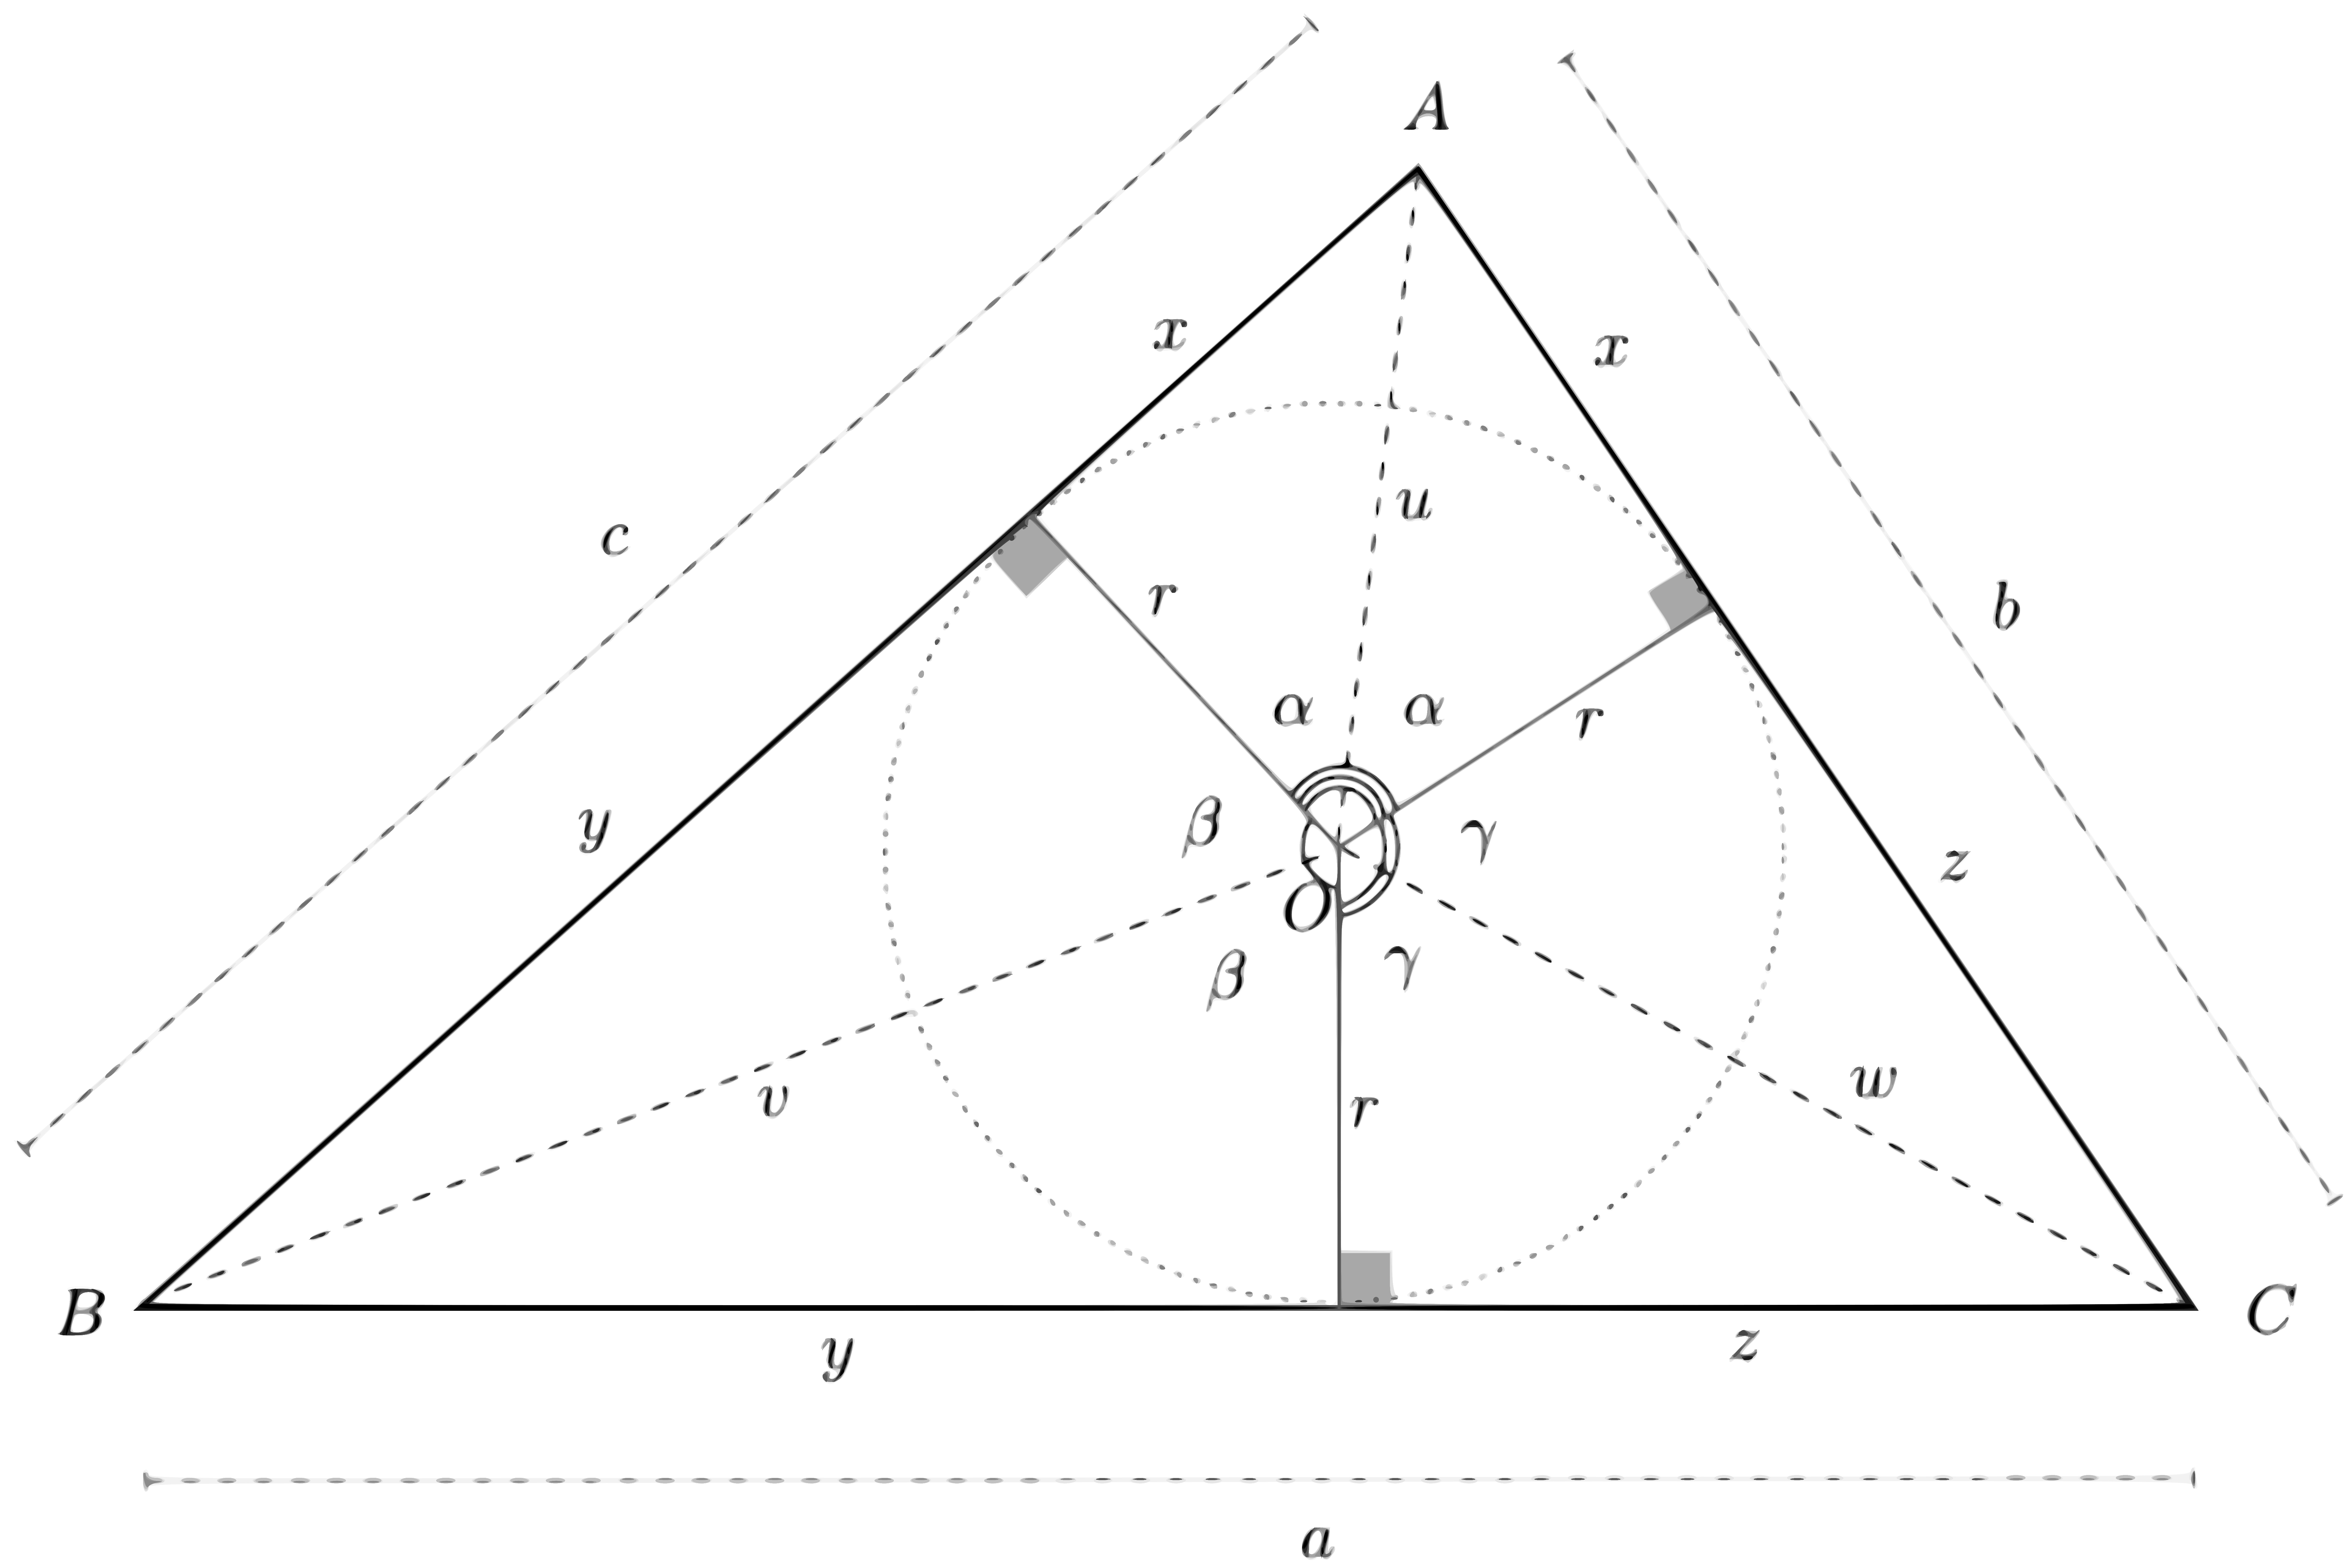
\includegraphics[width=0.68\linewidth]{secGD/figures/heron.png}
			\end{center}
			\caption{Formula de Herão: uma demonstração usando números complexos. \cite{libertiSixGemsDGHistory}}
			\label{fig:heron}
		\end{figure}
		
		\noindent Primeiro, nota-se que $2\alpha + 2\beta + 2\gamma = 2\pi$, o que implica $\alpha + \beta + \gamma = \pi$. Depois, as seguintes identidades complexas são facilmente verificadas na Figura~\ref{fig:heron}:
		$$ r+ix = ue^{i\alpha}, \quad r+iy = ve^{i\beta}, \quad r+iz = we^{i\gamma}.$$
		
		\noindent Isso implica que:
		
		$$(r+ix)(r+iy)(r+iz) \ =\ (uvw)e^{i(\alpha+\beta+\gamma)} \ =\ uvwe^{i\pi},$$
		
		\noindent e, conhecendo a identidade de Euler $e^{i\pi} = -1$, 
		
		$$uvwe^{i\pi} \ =\ -uvw.$$
		
		\noindent Como $-uvw$ é um número real, a parte imaginária de $(r+ix)(r+iy)(r+iz)$ deve ser zero. Expandindo o produto e rearranjando seus termos, tem-se que $r^2(x+y+z) = xyz$. Ao isolar $r$, caí-se na raiz não negativa
		
		\begin{equation}
			r = \sqrt{\frac{xyz}{x+y+z}}.
			\label{eq:herondemo}
		\end{equation}
		
		\noindent Pode-se escrever o semiperímetro do triângulo $ABC$ como $s=\frac{1}{2}(a+b+c)=\frac{1}{2}(y+z+x+z+x+y) = x+y+z$. Além disso,
		
		$$s-a=x+y+z-y-z=x, \quad s-b = x+y+z-x-z = y, \quad s-c = x+y+z-x-y=z,$$
		
		\noindent portanto $xyz = (s-a)(s-b)(s-c)$, implicando que a Equação~\ref{eq:herondemo} se torna:
		
		$$r = \sqrt{\frac{(s-a)(s-b)(s-c)}{s}}.$$
		
		\noindent Então escreve-se a área $A$ do triangulo $ABC$ como soma das áreas dos triângulos $AOB$, $BOC$ e $COA$, gerando
		
		$$A = \frac{1}{2}(ra + rb+ rc) \ =\ r\frac{a+b+c}{2} \ =\ rs \ =\ \sqrt{s(s-a)(s-b)(s-c)}.$$
	\end{proof}
\end{teorema}

Pode-se dizer que esse foi o nascimento da \textit{Geometria de Distâncias} (\textit{Distance Geometry}, ou DG) \cite{libertiSixGemsDGHistory}.
\\

Algumas centenas de anos depois, em 1841, Arthur Cayley (1821 a 1895) generalizou a~\ref{eq:Herão} através da construção de um determinante que calcula o conteúdo (volume $n$-dimensional) de um \textit{Simplex}\footnote{Um simplex é uma generalização do conceito de triangulo a outras dimensões, i.e., é a envoltória convexa ao redor dos pontos: O \textit{0-simples} é um ponto, \textit{1-simplex} é um segmento de reta, \textit{2-simplex} é um triangulo e o \textit{3-simplex} é um tetraedro.} em qualquer dimensão \cite{cayley1841HaronGD, douglasGD}. Um século depois, em 1928, o matemático austríaco Karl Menger (1902 a 1985) re-organizou as ideias de Cayley e trabalhou em uma construção axiomática da geometria através de distâncias \cite{mengerDeterminante} --- originando a alteração no nome do determinante de Cayley para como é conhecido hoje: \textit{Determinante de Cayley-Menger}.  

\begin{definicao}[Determinante de Cayley-Menger]
	O \emph{Determinante de Cayley-Menger} de um conjunto de $n+1$ pontos $p_0,p_1,\dots,p_n$, onde $d_{ij}$ corresponde a distância entre os pontos $p_i$ e $p_j$, é dado por
	\begin{equation}\tag{Determinante de Cayley-Menger}
		D_{CM}(p_0,\dots,p_n) = 
		\begin{vmatrix}
			0 & d^2_{01} & \ldots & d^2_{0n} & 1\\ 
			d^2_{01} & 0 & \ldots & d^2_{1n} & 1\\ 
			\vdots & \vdots & \ddots & \vdots & \vdots\\ 
			d^2_{0n} & d^2_{1n} & \ldots & 0 & 1\\ 
			1 & 1 & \ldots & 1 & 0\\ 
		\end{vmatrix}.
		\label{determinanteCayleyMenger}
	\end{equation}
\end{definicao}

\begin{lema}
	Considere um $K$- simplex em $\mathbb{R}^K$ de vértices $x_i$, $i = 0,\dots,k$, cujas coordenadas $x_i^j$ ($j = 1,\dots,k$) são conhecidas. O \textit{Volume Orientado} $\mathbb{V}$ desse $K$-simplex é dado pela expressão
	\begin{equation}
		\mathbb{V} = \frac{1}{K!} 
		\begin{vmatrix}
			x_0^1 & x^2_{0} & \ldots & x^K_{0} & 1\\ 
			x^1_{1} & x^2_1 & \ldots & x^K_{1} & 1\\ 
			\vdots & \vdots & \ddots & \vdots & \vdots\\ 
			x^1_{K} & x^2_{K} & \ldots & x_K^K & 1\\ 
		\end{vmatrix}.
		\label{eq:volumeOrientado}
	\end{equation}

	\begin{proof}
		(\cite{douglasGD}). Em $\mathbb{R}^2$, três pontos não colineares determinam um triângulo. Se esses pontos possuem coordenadas as coordenadas $x_0, x_1$ e $x_2$, utilizando Geometria Analítica, sabe-se que a área orientada do paralelogramo definido pelos vetores coluna $x_1-x_0$ e $x_2-x_0$ é dada por
		
		$$ A = \begin{vmatrix}
			(x_1-x_0)^T \\
			(x_2-x_0)^T \\
		\end{vmatrix}.$$
		
		\noindent Portanto, a área orientada $\mathbb{V}_2$ do triangulo induzido pelos vetores $x_1-x_0$ e $x_2-x_0$ é
		$$\mathbb{V}_2 = \frac{1}{2}|A|.$$
		
		\noindent De forma semelhante, quatro pontos afimente independentes em $\mathbb{R}^3$ formam um tetraedro. Se a coordenadas de seus pontos forem $x_0,x_1,x_2$ e $x_3$, o volume orientado $\mathbb{V}_3$ deste tetraedro é dado por 
		
		$$ \mathbb{V}_3 = \frac{1}{6}\begin{vmatrix}
			(x_1-x_0)^T \\
			(x_2-x_0)^T \\
			(x_3-x_0)^T \\
		\end{vmatrix}.$$
		
		\noindent Assim como em \cite{hanson1994geometry}, a fórmula para o cálculo de um volume orientado $\mathbb{V}_n$ de um $n$-simplex pode ser generalizada (por indução) a partir daqui. Um fator multiplicativo inversamente proporcional a $K!$ aparece na expressão, de modo a ter-se
		
		$$\mathbb{V}_K = \frac{1}{K!}\begin{vmatrix}
			(x_1-x_0)^T \\
			(x_2-x_0)^T \\
			\vdots \\
			(x_K-x_0)^T \\
		\end{vmatrix}.$$
		
		\noindent Ainda, pela expansão de Laplace, tem-se que
		
		$$\mathbb{V}_K = \frac{1}{K!}\begin{vmatrix}
			(x_0)^T & 1\\
			(x_1-x_0)^T & 0\\
			(x_2-x_0)^T & 0\\
			\vdots & \vdots\\
			(x_K-x_0)^T & 0\\
		\end{vmatrix},$$
		
		\noindent e pode-se somar a primeira linha as outras, sem alterar o valor do determinante, chegando ao nosso objetivo:
		
		$$\mathbb{V}_K = \frac{1}{K!}\begin{vmatrix}
			(x_0)^T & 1\\
			(x_1)^T & 1\\
			(x_2)^T & 1\\
			\vdots & \vdots\\
			(x_K)^T & 1\\
		\end{vmatrix} \quad = \quad \frac{1}{K!} 
		\begin{vmatrix}
			x_0^1 & x^2_{0} & \ldots & x^K_{0} & 1\\ 
			x^1_{1} & x^2_1 & \ldots & x^K_{1} & 1\\ 
			x^1_{2} & x^2_2 & \ldots & x^K_{2} & 1\\ 
			\vdots & \vdots & \ddots & \vdots & \vdots\\ 
			x^1_{K} & x^2_{K} & \ldots & x_K^K & 1\\ 
		\end{vmatrix}.$$
	\end{proof}
\end{lema}

Com isso, pode-se enunciar o seguinte resultado:

\begin{teorema}
	Considere os $K+1$ pontos $p_0, \dots, p_K$ que definem os vértices de um $K$-simplex em um espaço euclidiano $K$-dimensional. Então, o quadrado do conteúdo $\mathbb{V}_K$ desse $K$-simplex é
	\begin{equation}
		\mathbb{V}_K^2(p_0, \dots, p_K) = \frac{(-1)^{K+1}}{(K!)^22^K} D_{CM}(p_0, \dots, p_K).
		\label{eq:volumeKdimensionalNSimplex}
	\end{equation}
	
	\begin{proof}(\cite{douglasGD}). Pelo Lema anterior, tem-se que 
		$$\mathbb{V} = \frac{1}{K!} 
		\begin{vmatrix}
			x_0^1 & x^2_{0} & \ldots & x^K_{0} & 1\\ 
			x^1_{1} & x^2_1 & \ldots & x^K_{1} & 1\\ 
			\vdots & \vdots & \ddots & \vdots & \vdots\\ 
			x^1_{K} & x^2_{K} & \ldots & x_K^K & 1\\ 
		\end{vmatrix}.
		$$
		
		\noindent Pode-se utilizar o modelo de \textit{Coordenadas Homogêneas} para descrever a matriz do determinante acima em um \textit{Hiperplano Afim} de uma dimensão superior, ao introduzirmos uma borda de zeros com um 1 na diagonal, o que não altera o valor do determinante. Obtêm-se, então
		
		\begin{equation}
			\mathbb{V} = \frac{1}{K!} 
			\begin{vmatrix}
				x_0^1 & x^2_{0} & \ldots & x^K_{0} & 1 & 0\\ 
				x^1_{1} & x^2_1 & \ldots & x^K_{1} & 1 & 0\\ 
				\vdots & \vdots & \ddots & \vdots & \vdots & \vdots\\ 
				x^1_{K} & x^2_{K} & \ldots & x_K^K & 1 & 0\\
				0 & 0 & \ldots & 0 & 0 & 1\\ 
			\end{vmatrix}.
			\label{eq:detA}
		\end{equation}
		
		\noindent Agora, permuta-se as duas últimas colunas da matriz (o que alterna o sinal do determinante) e, como det($A$) $=$ det($A^T$), pode-se tomar a transposta, da forma
		
		\begin{equation}
			\mathbb{V} = -\frac{1}{K!} 
			\begin{vmatrix}
				x_0^1 & x^1_{1} & \ldots & x^1_{K} & 0\\ 
				x^2_0 & x^2_1 & \ldots & x^2_{K} & 0\\ 
				\vdots & \vdots & \ddots & \vdots & \vdots \\ 
				x^K_{0} & x^K_{1} & \ldots & x_K^K & 0\\
				0 & 0 & \ldots & 0 & 0 \\ 
				1 & 1 & \ldots & 1 & 1 \\ 
			\end{vmatrix}.
			\label{eq:detAT}
		\end{equation}
		
		\noindent Sabendo que det($AA^T$) $=$ det($A$)det($A^T$), e que ambas a matriz do determinante acima tem dimensão $(K+2)\times (K+2)$, pode-se multiplicar a Equação~\ref{eq:detA} pela Equação~\ref{eq:detAT} e obter
		
		\begin{equation*}
			\mathbb{V}^2 = -\left( \frac{1}{K!}\right)^2 
			\begin{vmatrix}
				x_0^Tx_0 & x^T_{0}x_1 & \ldots & x^T_{0}x_K & 1\\ 
				x_1^Tx_0 & x^T_1x_1 & \ldots & x^T_{1}x_K & 1\\ 
				\vdots & \vdots & \ddots & \vdots & \vdots \\ 
				x^T_{K}x_0 & x^T_{K}x_1 & \ldots & x_T^Kx_K & 1\\
				1 & 1 & \ldots & 1 & 0\\ 
			\end{vmatrix}.
		\end{equation*}
		
		\noindent E, sabendo que $x_i^Tx_j = \frac{1}{2}(x_i^Tx_i + x_j^Tx_j - d_{ij}^2)$, pode-se alterar cada linha $i$, com $0 \leq i\leq K$, pela soma dela com a última linha multiplicada por $-\frac{1}{2}x^T_ix_i$ (o que não altera o valor do determinante, por ser uma operação elementar). Também, pode-se fazer processo semelhante com as colunas: substituir cada coluna $j$, com $0\leq j\leq K$, pela sua soma coma multiplicação da última coluna por $-\frac{1}{2}x^T_jx_j$. O que gera
		
		\begin{equation*}
			\mathbb{V}^2 = -\left( \frac{1}{K!}\right)^2 
			\begin{vmatrix}
				-\frac{1}{2}d^2_{00} & -\frac{1}{2}d^2_{01} & \ldots & -\frac{1}{2}d^2_{0K} & 1\\ 
				-\frac{1}{2}d^2_{01} & -\frac{1}{2}d^2_{11} & \ldots & -\frac{1}{2}d^2_{1K} & 1\\ 
				\vdots & \vdots & \ddots & \vdots & \vdots \\ 
				-\frac{1}{2}d^2_{0K} & -\frac{1}{2}d^2_{1K} & \ldots & -\frac{1}{2}d^2_{KK} & 1\\
				1 & 1 & \ldots & 1 & 0\\ 
			\end{vmatrix}.
		\end{equation*}
		
		\noindent Visto que ao multiplicar uma coluna da matriz do determinante por um escalar $\alpha$, o próprio determinante é multiplicado por $\alpha^{-1}$, pode-se multiplicar as primeira $K+1$ colunas da matriz acima por -2, obtendo:
		
		\begin{equation*}
			\mathbb{V}^2 = \frac{-1}{(K!)^2}\left( -\frac{1}{2}\right)^{K+1} 
			\begin{vmatrix}
				d^2_{00} & d^2_{01} & \ldots & d^2_{0K} & 1\\ 
				d^2_{01} & d^2_{11} & \ldots & d^2_{1K} & 1\\ 
				\vdots & \vdots & \ddots & \vdots & \vdots \\ 
				d^2_{0K} & d^2_{1K} & \ldots & d^2_{KK} & 1\\
				-2 & -2 & \ldots & -2 & 0\\ 
			\end{vmatrix}.
		\end{equation*}
		
		\noindent Como uma propriedade semelhante existe para multiplicações de linhas da matriz de um determinante, pode-se dividir a última linha da matriz anterior por -2. Também, ajeitando os coeficientes, tem-se
		
		\begin{equation*}
			\mathbb{V}^2 = (-2) \frac{-1}{(K!)^2}\frac{(-1)^{K+1}}{2^{K+1}} 
			\begin{vmatrix}
				d^2_{00} & d^2_{01} & \ldots & d^2_{0K} & 1\\ 
				d^2_{01} & d^2_{11} & \ldots & d^2_{1K} & 1\\ 
				\vdots & \vdots & \ddots & \vdots & \vdots \\ 
				d^2_{0K} & d^2_{1K} & \ldots & d^2_{KK} & 1\\
				1 & 1 & \ldots & 1 & 0\\ 
			\end{vmatrix}.
		\end{equation*}
		
		\noindent Por fim, como a distância $d_{ii} = 0$ para qualquer valor de $i$ (pela definição de métrica), obtêm-se a expressão final, tal qual como desejava-se,
		
		\begin{equation*}
			\mathbb{V}^2 = \frac{(-1)^{K+1}}{2^{K}(K!)^2} 
			\begin{vmatrix}
				0 & d^2_{01} & \ldots & d^2_{0K} & 1\\ 
				d^2_{01} & 0 & \ldots & d^2_{1K} & 1\\ 
				\vdots & \vdots & \ddots & \vdots & \vdots \\ 
				d^2_{0K} & d^2_{1K} & \ldots & 0 & 1\\
				1 & 1 & \ldots & 1 & 0\\ 
			\end{vmatrix} \quad = \quad \frac{(-1)^{K+1}}{2^{K}(K!)^2} D_{CM}(p_0,\dots,p_K).
		\end{equation*}
	\end{proof}	
\end{teorema}

Mas foi só com Leonard Blumenthal (1901 a 1984) que, em 1953, o termo Geometria de Distâncias foi cunhado --- com a publicação de seu livro \textit{``Theory and Applications of Distance Geometry''} \cite{Blumenthal:53}.
Blumenthal dedicou sua vida de trabalho para clarificar, organizar e traduzir as obras originais em alemão. Ele acreditava que o problema mais importante nesta área era o \textit{``Problema de Subconjunto''} (ou \textit{Subset Problem}, originalmente), que consistia em encontrar condições necessárias e suficientes a fim de decidir quando uma matriz simétrica era, de fato, uma \textit{Matriz de Distâncias}\footnote{Seja o par $(\mathcal{X}, d)$ um Espaço Métrico, onde $\mathcal{X} = \{x_1, \dots, x_n\}$. Uma \textit{Matriz de Distância sobre $\mathcal{X}$} é uma matriz quadrada $D_{n\times n} = (d_{uv})$ onde, para todo $u,v \leq n$, temos $d_{uv} = d(x_u,x_v)$.}. Uma restrição desse problema à métrica euclidiana chama-se \textit{Problema de Matrizes de Distâncias Euclidianas} (ou EDMP, do inglês \textit{Euclidean Distance Matrix Problem}), como segue definida:

\begin{definicao}[Problema de Matrizes de Distâncias Euclidianas]
	\label{EDMP}
	Determinar se, para uma dada matriz quadrada $D_{n\times n} = (d_{ij})$, existe um inteiro $K$ e um conjunto $\{p_1, \dots, p_n \}$ de pontos em $\mathbb{R}^K$ tal que $d_{ij} = \lVert p_i - p_j\rVert$ para todo $i,j \leq n$.
\end{definicao}

Condições necessárias e suficientes para que uma matriz seja, de fato, uma matriz de distância euclidiana são dados em \cite{EDMPResolucao}. Para isso, apresenta-se um teorema onde se utiliza o~\ref{determinanteCayleyMenger} na criação de duas condições afirmando que, afim de $D_{n\times n}$ ser uma matriz de distâncias euclidianas, deve haver um $K$-simplex $S$ de referência com conteúdo $v_K \neq 0$ em $\mathbb{R}^K$ e que todos os $(K+1)$-simplex e $(K+2)$-simplex contendo $S$ como uma das faces devem estar contidos em $\mathbb{R}^K$ \cite{carlileGDandAplications}.
\\

Blumenthal percebeu a importância em se respeitar as restrições métricas estabelecidas pelas matrizes de distâncias.
\\

\begin{chapquote}{Blumenthal, \textit{Theory and Applications of Distance Geometry} \cite{Blumenthal:53}}
	``Quando temos como dado um conjunto de distâncias entre pares de pontos, a geometria das distâncias pode dar uma dica para encontrar um conjunto de coordenadas correto para pontos no espaço Euclideano tridimensional, satisfazendo as restrições de distâncias dadas.''
\end{chapquote}

Pode-se dizer que resolver o Problema de Matrizes de Distâncias Euclidianas está intimamente relacionado com descobrir as coordenadas dos pontos que definem suas distâncias. Perceba que este é um problema inverso, onde o ``problema direto'' correspondente é calcular distâncias associadas a pares de pontos dados. Note que este estudo tem enorme aplicabilidade.
\\

Adiante, em 1979, Yemini (professor emérito de Ciência da Computação na Universidade de Columbia) foi o primeiro a flexibilizar a definição do EDMP ao considerar um conjunto de distâncias esparso \cite{Yemini:79} --- \textit{i.e.}, que não se tem todas as distâncias dadas a priori. Com isso, introduziu-se o que se chamou de \textit{Problema Posição - Localização}, onde deseja-se calcular a localização de todos os objetos imersos em um espaço geográfico. 
Com isso, foi possível reformular o problema fundamental de Geometria de Distâncias, o qual pode ser caracterizado de forma mais moderna pela utilização da Teoria de Grafos\footnote{Se não estiver familiarizado com o conceito de grafo, ele é introduzido no Apêndice~\ref{ap:grafos}}.

\subsection{O Problema Fundamental}

\begin{definicao}[Realização]
	Uma \emph{realização} de um grafo $G = (V,E)$ é uma função que mapeia o conjunto de vértices $V$ para um espaço euclidiano de alguma dimensão dada.
\end{definicao}

\begin{definicao}[Problema de Geometria de Distâncias]
	Dados um grafo simples, ponderado e conectado $G = (V, E, d)$ e um inteiro $K>0$, encontre uma realização $x: V \longrightarrow \mathbb{R}^K$ tal que:
	\begin{equation}
		\forall \{u,v\} \in E, \hspace{0.5cm} \lVert x(u) - x(v) \rVert = d(u,v). \label{eq:DGP}
	\end{equation}	
\end{definicao}

Desde que uma realização seja encontrada, também dá-se a ela o nome de \textit{solução} do problema de geometria de distâncias (que abreviaremos DGP). Por simplicidade, adotaremos o abuso de notação $x_u$ e $d_{uv}$ no lugar de $x(u)$ e $d(u,v)$, respectivamente.
\\

A principal diferença desta definição para o EDMP está acerca de que uma matriz de distância essencialmente representa um \textit{Grafo Ponderado Completo}. Em contraponto, o DGP não empoe qualquer estrutura em $G$\footnote{A menos, é claro, no que diz respeito a seus vértices estarem conectados. Porém, caso $G$ não seja conectado, então ele consiste de um conjunto de diferentes subgrafos conectados, donde, a fim de solucionar o DGP, pode-se realizar cada subgrafo separadamente.}, seguindo o conceito de matriz esparsa estabelecido por Yemini.

Também, como utiliza-se na equação~\ref{eq:DGP} a norma euclidiana $\lVert$ $\cdot$ $\rVert$ como métrica, donde pode-se reescrever esta equação como

\begin{equation*}
	\forall \{u,v\} \in E, \hspace{0.5cm} \sqrt{\sum_{i=1}^{K}(x_{ui} - x_{vi})^2} = d_{uv}.
\end{equation*}

Como a definição de métrica garante a positividade das distâncias, pode-se esconder a raiz quadrada na equação acima, \textit{i.e.}

\begin{equation}
\forall \{u,v\} \in E, \hspace{0.5cm} \sum_{i=1}^{K}(x_{ui} - x_{vi})^2 = d_{uv}^2.
\label{eq:DGPSistemaQuadratico}
\end{equation}

\subsection*{Os Diferentes Problemas em DG}

Em 2014, Leo Liberti \textit{et al.} publicaram um ótimo compendio sobre a \textit{Geometria de Distâncias Euclidianas e suas Aplicações} e, em particular, desenvolveram um estudo  taxonômico muito interessante sobre os problemas clássicos da área. No que se segue, devido a grande quantidade de siglas e variações dentro de DG, apresenta-se parte desse estudo, visando organizar os conceitos. 
\\

As principais aplicações em DG são no \textit{Calculo de Estruturas Moleculares} \cite{crippen:DistancesAndMolecularConformation}, na \textit{Localização de Sensores em Redes Sem Fio} (\textit{Wireless Sensor Network Localization}, ou WSNL) \cite{yemini1978positioning}, em \textit{Cinemática Inversa} (\textit{Inverse Kinematic}, ou IK) \cite{cinematicaInversa} e em \textit{Escalonamento Multidimensional} (\textit{Multidimensional Scaling}, ou MDS) \cite{multidimensionalScaling}.

\subsubsection{Escalonamento Multidimensional}

O problema de \textit{Escalonamento Multidimensional} (\textit{Multidimensional Scaling}, ou MDS)
é definido como: Dado um conjunto $X$ de vetores, encontre um conjunto $Y$ de vetores com menor dimensão (com $|X| = |Y|$) tal que a distância entre cada $i$-ésimo e $j$-ésimo vetores de $Y$ tenham, aproximadamente, a mesma distância que seus pares de vetores correspondentes em $X$.

Esse problema é muito aplicado na analise de dados em Big Data \cite{libertiEDG}. É um meio de facilitar a visualização do nível de similaridade entre casos individuais --- que não necessariamente precisam ter uma conexão aparente --- em um conjunto de dados. Pode-se usá-lo, por exemplo, para visualizar em uma escala bidimensional ($\mathbb{R}^2$) a evolução da locomoção de animais no espaço tridimensional utilizando dados de séries temporais (espaço em diferentes tempos, logo, dados em $\mathbb{R}^4$).

\subsubsection{Conformações Moleculares}

Existe uma relação muito forte com a forma geométrica das moléculas e suas funções em organismos vivos \cite{bioquimicaLehninger}. Projetar drogas para curar uma doença específica se trata basicamente de conhecer o que uma certa proteína pode fazer em um organismo \cite{libertiEDG}. Proteínas se ligam em outras moléculas através do equilíbrio de forças agindo entre elas\footnote{Ou seja, o equilíbrio da energia potencial das moléculas, proporcional, principalmente, as variações nos comprimentos das ligações covalentes, as variações nos ângulos entre duas ligações covalentes consecutivas, as rotações sobre as ligações covalentes e as interações de van der Waals e interações eletrostáticas entre átomos \cite{carlileTese}.}, portanto, suas ligações dependem do seu formato. 

Proteínas são constituídas por um grande conjunto de átomos e, alguns pares destes, trocam ligações químicas --- sabe-se quais são esses átomos através de experimentos de cristalografia \cite{ramachandran1974MolStructure}. Então, se os átomos de uma molécula forem rotulados da forma $1,3,4,\dots,n$, é possível inferir: 
\begin{itemize}
	\item O conjunto de ligações $\{u,v\}$, onde $u,v$ são átomos em $\{1,\dots,n\}$;
	\item A distância entre $u$ e $v$ (para cara par ligado);
	\item O ângulo interno $\theta_v$ definido por duas ligações $\{u,v\}$ e $\{v,w\}$, com um átomo $v$ em comum.
\end{itemize} 

Além desses dados, também é possível obter mais informações a partir de experimentos mais sofisticados, como a \textit{Ressonância Magnética Nuclear} (RMN). Neste experimento é escolhida uma faixa de radiofrequência para bombardear uma amostra que está imersa em um campo magnético bastante intenso. Dependendo da radiofrequência utilizada (costuma-se usar a do hidrogênio), alguns núcleos atômicos irão absorver energia e outros não. Caso atinja-se uma frequência exata de ressonância dentro destes núcleos atômicos, é possível medir essa ressonância como um sinal de radiofrequência enviado dos núcleos atômicos para calcular distâncias entre átomos próximos, com distâncias menores que 5\AA.
\\

De posse dessas informações, deseja-se realizar (localizar) todos os átomos da molécula. Esse problema, com todas as informações moleculares disponíveis, denomina-se \textit{Estrutura Proteica a Partir de Dados Brutos} (\textit{Protein Structure from Raw Data}, ou PSRD). 
Em particular, como as coordenadas atômicas pertencem ao $\mathbb{R}^3$, há uma particularização do DGP para o caso molecular chamado \textit{Problema de Geometria de Distâncias Moleculares} (\textit{Molecular DGP}, ou MDGP). Trata-se do DGP com $K = 3$ fixo.

\subsubsection{Localização de Sensores}

O \textit{Problema de Localização de Sensores em Rede sem Fio} (ou \textit{WSNL Problem}) surge quando é necessário localizar um conjunto de objetos equipados com sensores eletrônicos capazes de medir distâncias entre si, geograficamente distribuídos, usando apenas medidas de distâncias entre pares destes objetos \cite{yemini1978positioning}. 

Por exemplo, \textit{smartphones} com WIFI ativo podem criar uma rede conhecida por \textit{Rede Ad-Hoc}, \textit{i.e.}, eles conseguem criar uma rede para comunicar-se entre si, de forma \textit{Peer-to-Peer}, sem a necessidade de uma torre central --- cada aparelho funciona como uma pequena torre, de forma que a distância entre os aparelhos não pode ser excessiva.
Dessa forma, os \textit{smartphones} podem estimar a distância $r$ de emparelhamento das suas conexões ao medir, por exemplo, qual a potência
\begin{equation}
	P = \frac{X}{r^n},
\end{equation}
de transmissão do sinal, inversamente proporcional a uma potência da distância $r$, onde $X$ e $n$ são constantes e obtidas experimentalmente \cite{savvides2001dynamic}.

Em essência, um problema do tipo WSNL segue a mesma definição do DGP, porém, com um subconjunto $A\subset V$ de vértices (chamados \textit{Âncoras}), onde os elementos de $A$ tem uma posição em $\mathbb{R}^k$ dada a priori --- isso é feito pois, normalmente, interessa saber a posição relativa de um objeto a outro, como é o caso do Sistema de Posicionamento Global, onde temos os satélites como âncoras e desejamos saber a posição dos aparelhos GPS em relação aos satélites.

Por motivos práticos --- semelhantes ao caso molecular --- as variações de interesse desse problema tem o $K$ fixo em $K= 2$ ou $K=3$. É comum, também, que se defina um WSNL como \textit{Solucionável} somente se seu grafo possua uma única realização válida --- noção conhecida como \textit{Globalmente Rígido}: Diz-se que um grafo é \textit{Globalmente Rígido} quando ele possui uma realização genérica $x$ e, para todas as outras realizações $x'$, $x$ é congruente a $x'$. 

\subsubsection{Dinâmicas em Cinemática Inversa}

Muito utilizada em robótica e animação computadorizada, a cinemática inversa cerne sobre mecanismos e seus movimentos rígidos, onde restringe-se os movimentos de forma a preservar a geometria do sistema. Sem o auxilio computacional e matemático a manipulação de mecanismos com muitos graus de liberdade  pode ser inviável: Imagine a manipulação manual de cem vértices em uma haste simulando o comportamento de um braço articulado em uma animação. Com o auxílio da DG, um animador pode apenas configurar a posição final de um pequeno grupo de vértices (como os da extremidade da aresta, por exemplo) e um algorítimo de cinemática inversa é capaz de verificar se aquela posição é ou não viável e, se viável, qual a realização de todo o conjunto de vértices em razão da posição configurada \cite{cinematicaInversa}.

Visando tal restrição mecânica, define-se o \textit{Problema de Cinemática Inversa} (\textit{Inverse Kinematic Problem}, ou IKP) como uma variação do WSNL --- logo, tem o objetivo de descobrir posições em relação a certos pontos previamente realizados --- com uma restrição no grafo que define o problema: deve ser um caminho simples com seus vértices finais sempre sendo âncoras.

\subsection{A Busca de uma Solução}

A abordagem mais simples, pode-se pensar, para encontrar um conjunto de soluções que satisfação a equação~\ref{eq:DGPSistemaQuadratico} é resolver o sistema de equações diretamente. Infelizmente, para $K \geq 2$, há evidencias de que uma solução de forma fechada onde todo componente de $x$ é expresso por raízes, não é possível \cite{carlileBook31Coloquio}. 

No entanto, pode-se reformular o problema como um Problema de Otimização Global, onde o objetivo é minimizar a soma dos \textit{Erros}\footnote{Em otimização, vê-se a equação~\ref{eq:DGP} de forma não exata: $\lVert x_u - x_v \rVert = d_{uv} + \varepsilon$, onde $\varepsilon$ é chamado \textit{Erro}. Ou seja, para minimizar o erro, precisa-se minimizar a expressão $f(x_u,x_v) = \lVert x_u - x_v \rVert - d_{uv}$.} entre as distâncias dadas a priori e as calculadas. Para isso, pode-se considerar uma única expressão que englobe todos os $n$ erros, da forma
\begin{equation}
	f(x_1,\dots,x_n) = \sum_{(i,j)\in E} \left(\lVert x_i - x_j \rVert^2 - d_{ij}^2\right)^2.
		\label{eq:problemaOtimizacaoGlobal1}
\end{equation}

Fica claro que encontrar uma solução para o DGP é equivalente a encontrar realizações $x_i \in \mathbb{R}^3$, $i=1,\dots,n$, tal que $f(x_1,\dots,x_n) = 0$. Visto que esta função se trata de uma soma de quadrados e que não há restrições nesse problema de Otimização Global, 0 é o valor mínimo de $f$. Deseja-se, portanto, minimizar a função $f: \mathbb{R}^n \longrightarrow \mathbb{R}$. Isto é,
\begin{equation}
	\label{eq:minDGP}
	\min_{x_i \in \mathbb{R}^n} f(x_1,\dots,x_n).
\end{equation}

No caso da métrica euclidiana, a Equação~\ref{eq:minDGP} torna-se

\begin{equation}
 \min_{x_j \in \mathbb{R}^n} \sum_{(u,v)\in E} \left(\sum_{i=1}^{K}(x_{ui} - x_{vi})^2 - d_{uv}^2\right)^2.
 \label{eq:DGPminEuclid}
\end{equation}

Perceba que a introdução conveniente de quadrados nas distâncias da função~\ref{eq:problemaOtimizacaoGlobal1} eliminou o calculo da raiz na norma euclidiana presente na Equação~\ref{eq:DGPminEuclid} --- uma otimização, principalmente por (i) multiplicação tem um custo computacional inferior ao da radiciação \cite{intructionsTableFog} e (ii) a radiciação pode apresentar alguns problemas numéricos para valores próximos de zero \cite{libertiMdgpContinousToDiscrete}. Portanto, a equação~\ref{eq:DGPminEuclid} tem como objetivo a minimização de um polinômio de múltiplas variáveis de grau quatro.
\\

Um dos desafios da Otimização Global é que muitos dos métodos existentes --- em especial, os mais eficientes --- não garantem que uma otimização \textit{global} será encontrada . Isso se dá pois podem existir muitos ótimos locais e, visto que os métodos de otimização continua dispõem apenas de informações locais, estes não conseguem diferenciá-los de um global \cite{carlileBook31Coloquio} (vide Figura~\ref{fig:minimoslocais}). %Em DG, a distribuição geométrica dos vértices do grafo está intimamente ligada com o comportamento da função objetivo --- donde, por exemplo, em WSNL, é interessante o estudo da distribuição geométrica dos sensores afim de melhorar a busca por ótimos globais \cite{eren2004rigidity}.
\begin{figure}[H]
	\begin{center}
		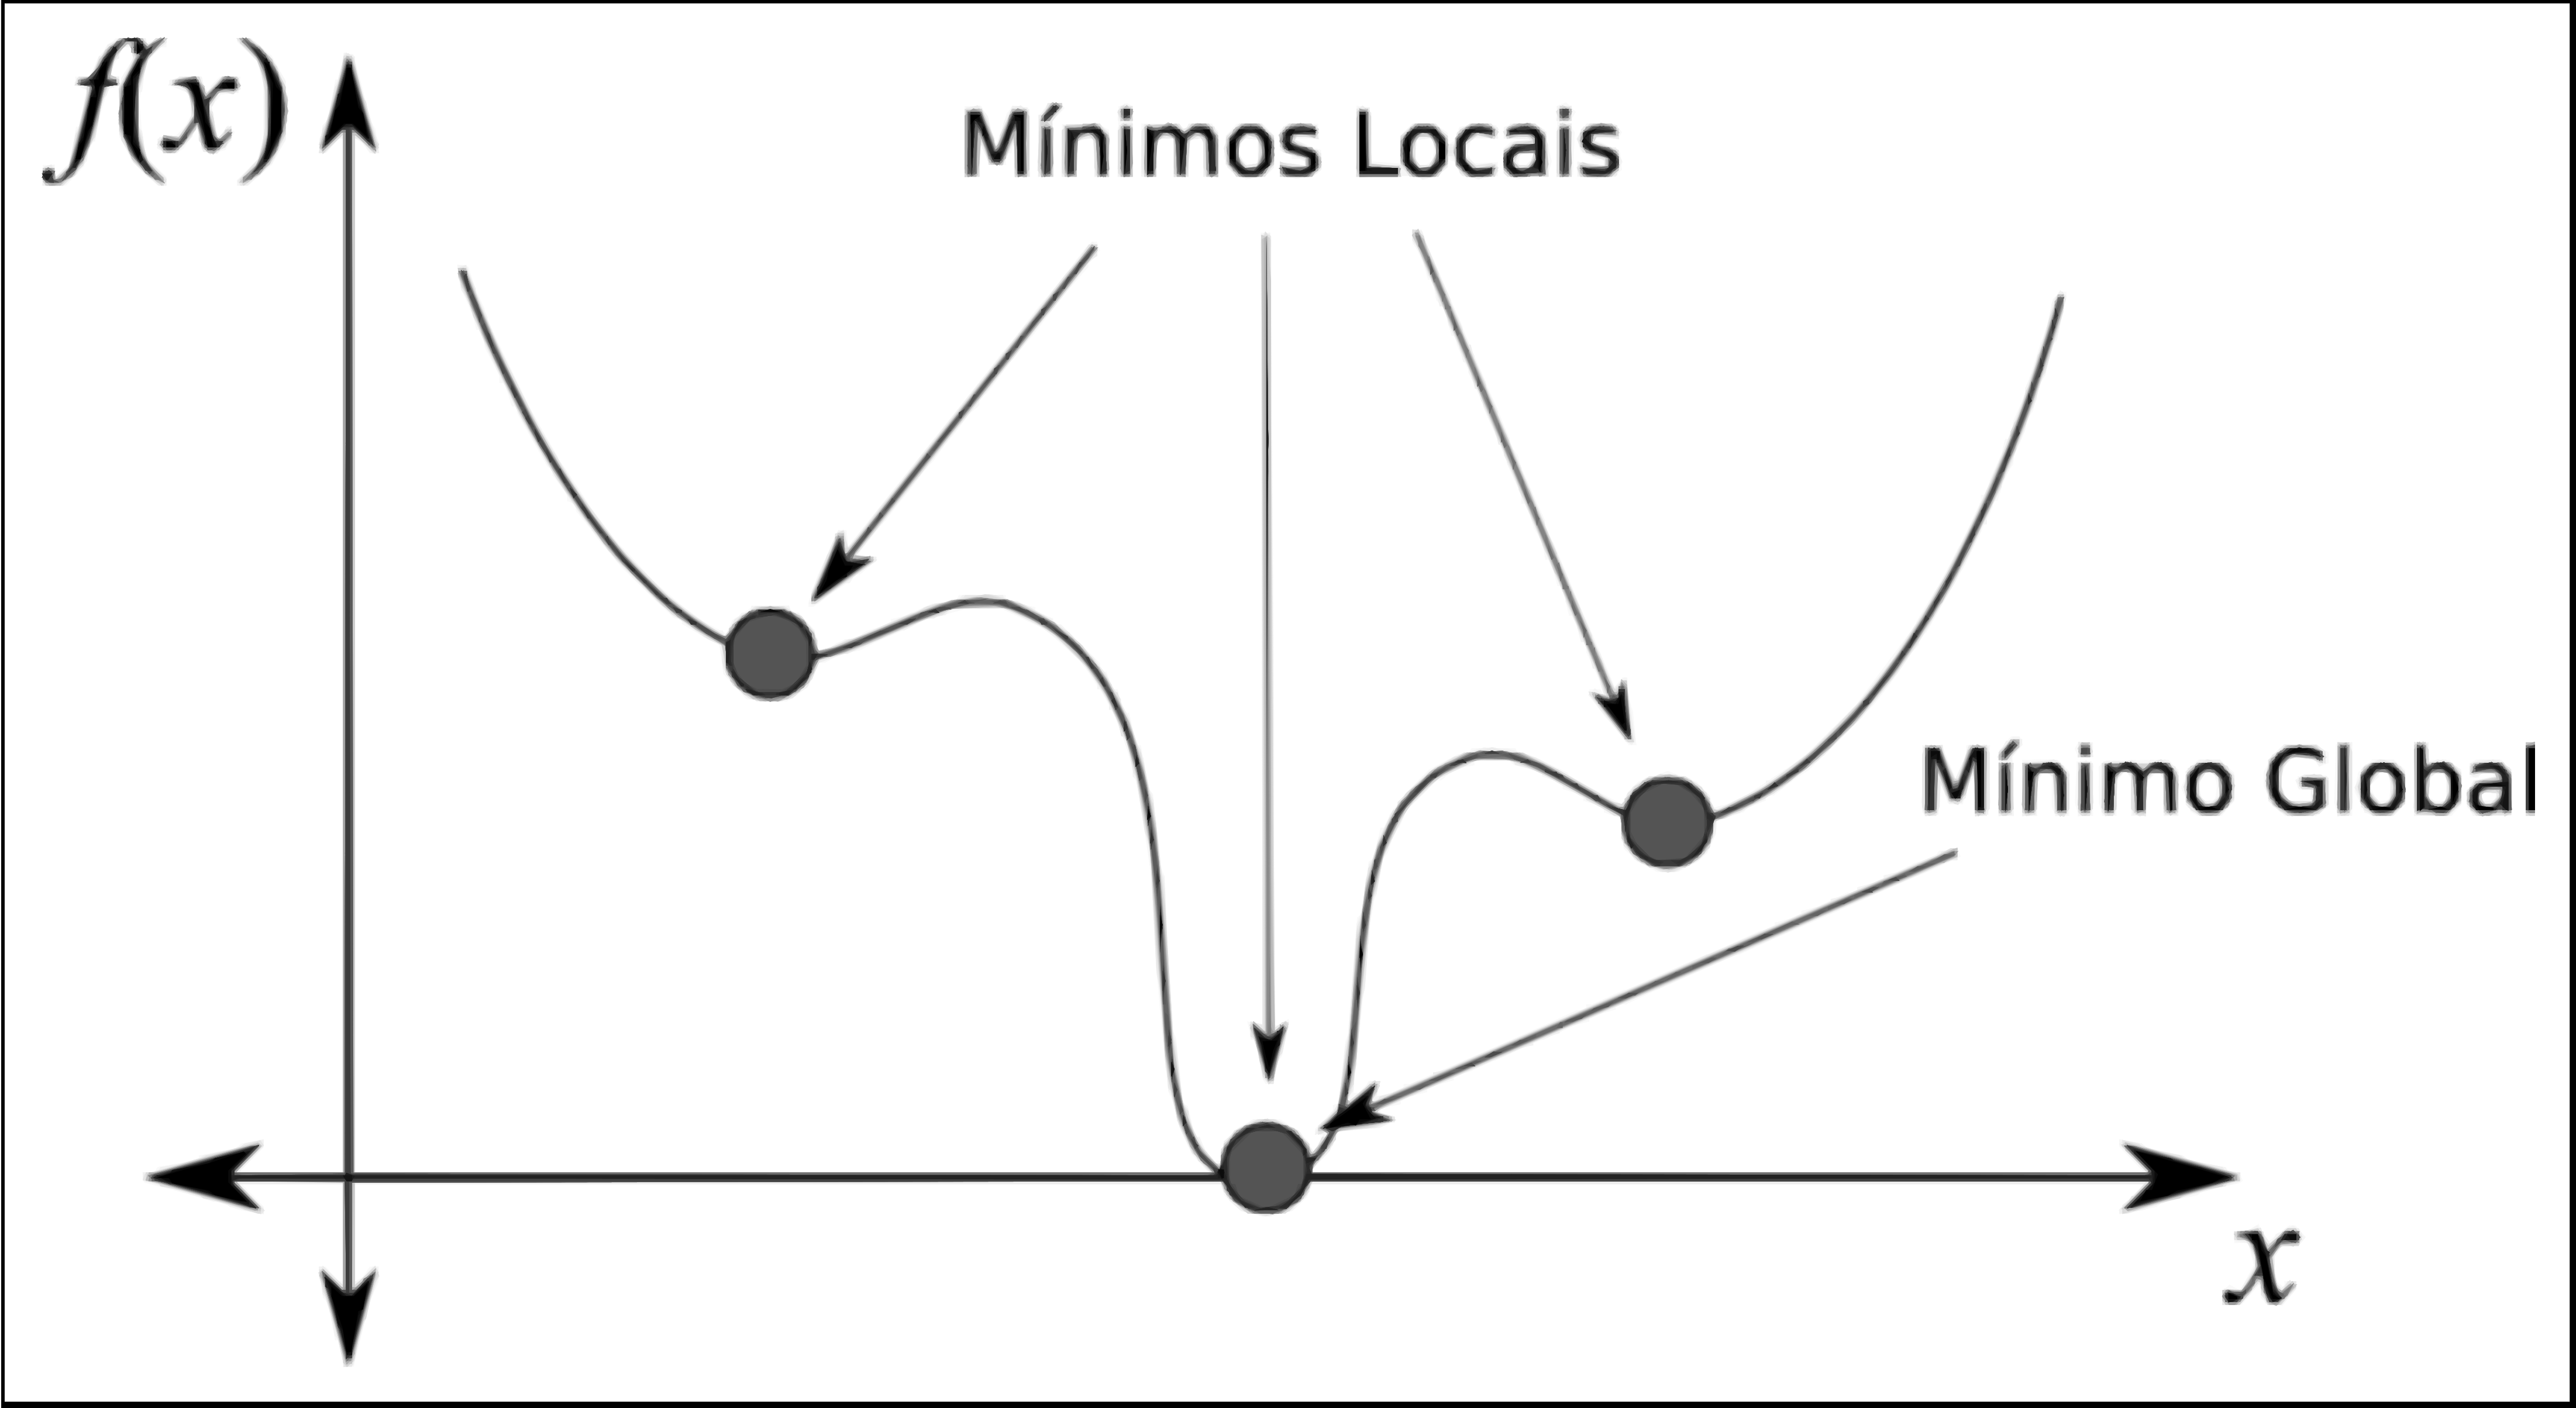
\includegraphics[width=0.47\linewidth]{secGD/figures/minimoslocais.png}
	\end{center}
	\caption{Diferenças entre mínimos locais e globais \cite{carlileBook31Coloquio}.}
	\label{fig:minimoslocais}
\end{figure}

Infelizmente, essa abordagem via Otimização Global é custosa do ponto de vista computacional --- como mostrado em \cite{carlileRecentAdvancesMDGP}, onde Carlile \textit{et. al.} citam as limitações dos métodos contínuos. Em 1979, Saxe demonstrou que resolver um DGP para qualquer dimensão --- \textit{i.e.}, para qualquer valor de $K$ --- tem a complexidade computacional da classe \textbf{NP}-Hard \cite{Saxe:79}. Em outras palavras, isso significa que a quantidade de mínimos locais de um DGP cresce exponencialmente proporcional a $|V|$ \cite{carlileIntroductionMDGP}. 

\subsubsection{A Quantidade de Soluções do Problema}

Seja $\bar{X} = \{x\; : \; V \rightarrow \mathbb{R}^K \; | \;x $ satisfaça (\ref{eq:DGP})$\}$ o conjunto de todas as soluções de uma instância DGP. Então, para qualquer transformação ortogonal $T$ de $\mathbb{R}^K$ (por exemplo, uma rotação ou translação) tem-se que, pela própria definição de ortogonalidade, se $x\in \bar{X}$ então $T(x) \in \bar{X}$. Define-se uma relação de equivalência $\sim$ sobre $\bar{X}$ como $\bar{x} \sim\bar{y}$ se e somente se existir uma transformação ortogonal $T$ tal que $\bar{y} = T\bar{x}$. Finalmente, define-se $X = \bar{X} /\sim$ e identifica-se a classe de equivalência de $X$ com um de seus representantes $x\in \bar{X}$. Em \cite{carlileRecentAdvancesMDGP} o conjunto $X$ é identificado como o conjunto de ``interesse'' para as soluções de uma instância DGP, pois este não leva em consideração soluções ``redundantes'' advindas de transformações ortogonais  --- e pode-se obter facilmente um número incontável de transformações ortogonais \cite{libertiMdgpContinousToDiscrete}.
\\

Mesmo que a definição da classe de equivalência acima possa remover uma quantidade não enumerável de soluções do problema, $|X|$ não é necessariamente finito. No geral, a quantidade de soluções do DGP depende da estrutura geométrica do grafo que a define: (i) podem não haver nenhuma realização; (ii) uma única realização; (iii) uma quantidade finita (não única) de realizações; ou, (iv) um número incontável de realizações. Perceba que, curiosamente, a quantidade de soluções de um DGP somente não pode ser um número infinito e enumerável --- sabe-se isso através de estudos em \textit{Geometria Algébrica Real} \cite{benedettireal}.\\
 
Ou seja, supondo que o conjunto solução de um DGP seja não vazio, sabe-se que ele é não enumerável ou finito. Se for não enumerável, pode-se tentar fazer uma busca contínua no espaço euclidiano --- como o algorítimo \textit{spatial Branch-and-Bound} (sBB), que faz uma $\epsilon$-aproximação para solucionar \textit{Nonlinear Programs} (NLPs) não convexos e \textit{Mixed-Integer NLPs} \cite{carlileGDandAplications}. Se for finito (normalmente o caso desejado), além de poder aplicar métodos de Otimização Global --- já definidos como custosos computacionalmente ---, pode-se explorar outras abordagens, como a Otimização Combinatória.

\subsection{Ferramentas Combinatórias na Solução do DGP}

Nesta seção, estuda-se sobre as condições que garantem a finitude do conjunto solução do problema ao analisar o espaço de busca por uma solução. Em particular, para um DGP definido em um espaço euclidiano de dimensão $K$, apresenta-se uma classe de grafos com propriedades muito interessantes: dos $(K+2)$-cliques, ou seja, dos grafos completos com dois vértices a mais do que o número de dimensões do seu espaço.

\subsubsection{Realização de Grafos Completos}

%Dado um $(K+1)$-clique com vértices não coincidentes (essa condição ficará mais clara ao decorrer desta seção), sabe-se que \textit{se ele possui} uma realização em $\mathbb{R}^{K-1}$, no geral, \textit{ela é única} a menos de rotações e translações \cite{libertiEDG, hendrickson1992conditions, connelly1991generic}. Porém, visto que para solucionar um DGP interessa uma solução em $\mathbb{R}^K$ ao invés de $\mathbb{R}^{K-1}$, pode-se usar um corolário um tanto óbvio da afirmação anterior: um $(K+2)$-clique com vértices não coincidentes tem, no máximo, uma realização única no espaço $\mathbb{R}^K$ (novamente, \textit{única} a menos de movimentos rígidos). 

Dependendo da estrutura do grafo que define um DGP, obter uma solução do problema pode garantir a unicidade desta solução \cite{eren2004rigidity}. Essa característica é de fundamental importância para algumas classes de problemas em DG, como o caso da WSNL, onde somente realizações únicas são consideradas como soluções. 

A seguir, baseado em \cite{libertiEDG} e \cite{trilaterationDong}, apresenta-se um método para calcular uma realização de um $(K+2)$-clique em $\mathbb{R}^K$.
\\

Considere um 3-clique ponderado com $V = \{1,2,3\}$, onde $d_{12} = d_{23} = 1$ e $d_{13} = 2$. Então, uma possível realização sobre a reta real $\mathbb{R}$ que satisfaça todas as distâncias é $x_1 = 0$, $x_2 = 1$ e $x_3 = 2$ (conforme Figura~\ref{fig:triexemplo}). Uma forma de obter o valor de $x_3$, dado os valores de $x_1$ e $x_2$ e as distâncias $d_{13}$ e $d_{23}$, é a \textit{Trilateração}.

\begin{figure}[H]
	\begin{center}
		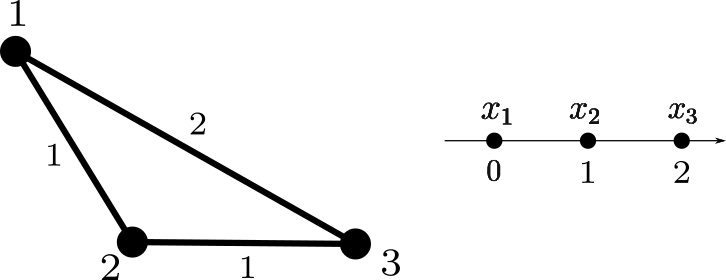
\includegraphics[width=0.55\linewidth]{secGD/figures/triExemplo.png}
	\end{center}
	\caption{Representação do Grafo (esquerda) e sua realização na reta (direita).}
	\label{fig:triexemplo}
\end{figure}

\subsubsection{Trilateração\label{sec:trilateration}}

 Vamos desenvolver este conceito a partir do exemplo mencionado acima. Se deseja encontrar as posições $x_1, x_2$ e $x_3$ de modo que satisfaçam as condições do DGP $d_{13} = \lVert x_3 - x_1\rVert = 2$ e $d_{23} = \lVert x_3 - x_2 \rVert = 1$. Usando a norma Euclidiana, $\lVert u-v\rVert^2 = (u-v)^2 = u^2 -2uv + v^2$, tem-se

\begin{equation}
	x_3^2 - 2x_1x_3 +x_1^2 = 4 \quad \textrm{e}
	\label{eq:trilateration1}
\end{equation}
\begin{equation}
x_3^2 - 2x_2x_3 +x_2^2 = 1. \quad
\label{eq:trilateration2}
\end{equation}

Subtraindo a equação~\ref{eq:trilateration2} da~\ref{eq:trilateration1}, obtém-se

\begin{equation*}
	2(x_1-x_2)x_3 = x_1^2 - x_2^2 - 3 \ \Rightarrow \ 2x_3 = 4 \ \Rightarrow \ x_3 = 2.
\end{equation*}

Pode-se generalizar esse exemplo facilmente para $(K+2)$-cliques em $\mathbb{R}^{K}$:
\\

Seja um DGP definido a partir de um $(K+2)$-clique $G$. Conhece-se previamente as posições $x_1, \dots, x_{k+1} \in \mathbb{R}^{K}$ de $K+1$ vértices de $G$ e deseja-se descobrir a posição $y\in\mathbb{R}^K$ do $(K+2)$-ésimo vértice de $G$. Pela definição do DGP, $y$ deve respeitar as $K+1$ equações quadráticas $\lVert x_j-y\rVert^2 = d_{j,K+2}^2$, $1\leq j\leq K+1$, com as $K$ componentes vetoriais de $y$ como incógnitas:

\begin{equation}
	\begin{cases} 
		\lVert y \rVert^2 -2x_1y + \lVert x_1\rVert^2 \ = \ d^2_{1,K+2}
		\\
		\qquad\qquad\qquad\quad\qquad \!\vdots
		\\
		\lVert y \rVert^2 -2x_{K+1}y + \lVert x_{K+1}\rVert^2 \ = \ d^2_{K+1,K+2}
	\end{cases}
	\label{eq:DGPsistemaEquacoes1}
\end{equation}

Subtraindo as $K$ primeiras equação do sistema de equações~\ref{eq:DGPsistemaEquacoes1} pela $(K+1)$-ésima equação

\begin{equation}
\begin{cases} 
\lVert y \rVert^2 -2x_1y + \lVert x_1\rVert^2 \ - (\lVert y \rVert^2 -2x_{K+1}y + \lVert x_{K+1}\rVert^2 )\; \; \ = \ d^2_{1,K+2} - \ d^2_{K+1,K+2}
\\
\qquad\qquad\qquad\quad\qquad\qquad\qquad\qquad\qquad\quad\qquad\quad \ \; \;\vdots
\\
\lVert y \rVert^2 -2x_Ky + \lVert x_K\rVert^2 \ - (\lVert y \rVert^2 -2x_{K+1}y + \lVert x_{K+1}\rVert^2 )\ = \ d^2_{K,K+2} - \ d^2_{K+1,K+2}
\end{cases}
\label{eq:DGPsistemaEquacoes3}
\end{equation}

pode-se formar um novo sistema, contendo $K$ equações com as mesmas $K$ incógnitas:

\begin{equation}
\begin{cases} 
2(x_1-x_{K+1}) \;\cdot y \ = \ \lVert x_1\rVert^2 - \lVert x_{K+1}\rVert^2 - d^2_{1,K+2} + d^2_{K+1,K+2} 
\\
\qquad\qquad\qquad\qquad\!\!\!\vdots
\\
2(x_{K}-x_{K+1}) \cdot y \ = \ \lVert x_{K}\rVert^2 - \lVert x_{K+1}\rVert^2 - d^2_{K,K+2} + d^2_{K+1,K+2} 
\end{cases}
\label{eq:DGPsistemaEquacoes2}
\end{equation}

Seja a matriz quadrada $A = (2(x_{ij} - x_{K+1j}))$, com $i,j \leq K$ como índices de linha e coluna (componentes vetoriais), respectivamente. Seja também o vetor coluna $b = (\lVert x_i\rVert^2 - \lVert x_{K+1}\rVert^2 - d^2_{i,K+2} + d^2_{K+1,K+2})^T$, onde $1 \leq i\leq K$. Então, pode-se reescrever o sistema de equações~\ref{eq:DGPsistemaEquacoes2} como o sistema linear

\begin{equation}
	Ay=b.
	\label{eq:DGPLinearSystem}
\end{equation}

Diferentes métodos para solução de sistemas lineares como a equação~\ref{eq:DGPLinearSystem} são encontrados na bibliografia \cite{AlgebraLinearElon} --- no geral, a escolha do melhor depende de propriedades da matriz $A$, como sobre sua singularidade, esparsidade, entre outros. Em particular, se $A$ não é uma matriz singular, então ela possui uma inversa $A^{-1}$. Pode-se, portanto, obter a posição do $(K+2)$-ésimo vértice fazendo

\begin{equation}
	Ay = b \quad \Rightarrow \quad A^{-1}Ay = A^{-1}b \quad \Rightarrow \quad y = A^{-1}b = x_{K+2}.
\end{equation}

No entanto, se A é singular, isso quer dizer que as linhas $a_i = x_i - x_{K+1}$ (para $i\leq K$) não são todas linearmente independentes \cite{AlgebraLinearElon}. Essa situação mostra algumas propriedades geométricas interessantes. Por exemplo, se $K=1$, significa que $x_1 - x_2 = 0 \ \Rightarrow \  x_1 = x_2$, ou seja, que o segmento entre $x_1$ e $x_2$ é um simples ponto. Como estamos imersos no $\mathbb{R}^{K} = \mathbb{R}$ (\textit{i.e.}, a reta real), geometricamente, a situação é que ou $x_3$ está posicionado a direita ou a esquerda de $x_1 = x_2$, mas não se pode escolher (veja a Figura~\ref{fig:retasingular}). Numericamente, é possível obter tais soluções ao utilizar a pseudoinversa de $A$ \cite{linearAlgebraNumericalTrefethen}.

\begin{figure}[H]
	\begin{center}
		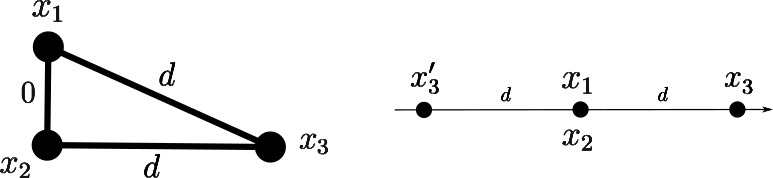
\includegraphics[width=0.7\linewidth]{secGD/figures/retasingular.png}
	\end{center}
	\caption{Representação da singularidade da matriz $A$ em $\mathbb{R}$.}
	\label{fig:retasingular}
\end{figure}

Não obstante, se $K = 2$, a singularidade de $A$ implica que o triangulo definido por $x_1$, $x_2$ e $x_3$ é apenas um segmento no plano (caso o rank de $A$ é 1) ou um simples ponto (caso o rank for 0). No primeiro caso, $x_4$ pode estar posicionado em ambos os lados da linha que contém o segmento e, no segundo caso, $x_4$ pode estar em qualquer um dos pontos formados pela circunferência com centro $x_1 = x_2 = x_3$ e raio $d_{14} = d_{24} = d_{34}$, conforme ilustra a Figura~\ref{fig:planosingular}. 
Essa característica geométrica vale para valores maiores de $K$: a singularidade de $A$ está relacionada a existência de vértices coincidentes e implica que há sempre múltiplas soluções para $x_{K+2}$.

\begin{figure}[H]
	\begin{center}
		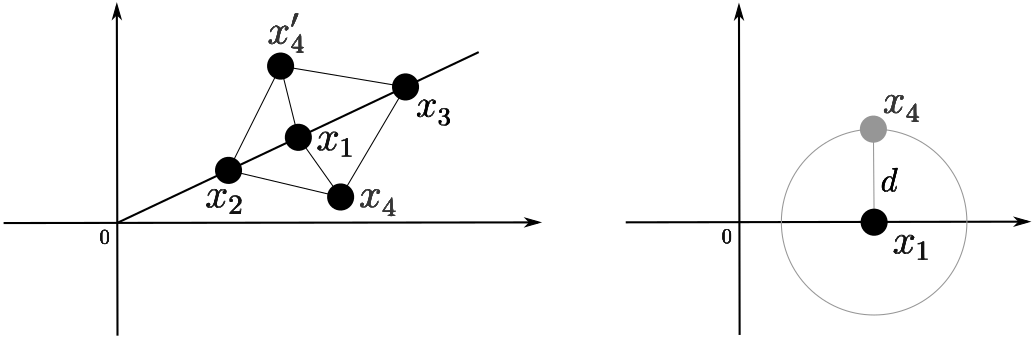
\includegraphics[width=0.85\linewidth]{secGD/figures/planosingular.png}
	\end{center}
	\caption{Representação da singularidade da matriz $A$ em $\mathbb{R}^2$. A esquerda, caso o rank de $A$ for 1 e, a direita, caso for 0.}
	\label{fig:planosingular}
\end{figure}

Por fim, é importante mencionar que a partir da equação~\ref{eq:DGPsistemaEquacoes1} podemos chegar no sistema linear~\ref{eq:DGPLinearSystem}, mas a recíproca não é verdadeira. Em particular, se o sistema~\ref{eq:DGPsistemaEquacoes1} tem uma solução, então o sistema~\ref{eq:DGPLinearSystem} tem a mesma solução. Porém, mesmo que o sistema~\ref{eq:DGPsistemaEquacoes1} não tenha solução, o sistema~\ref{eq:DGPLinearSystem} sempre terá uma solução única --- desde que $A$ não seja singular. Sendo assim, para verificar a factibilidade de uma solução $x_{K+2}$ advinda do sistema linear~\ref{eq:DGPLinearSystem}, deve-se verificar se as distâncias aos $K+1$ vértices foram respeitadas --- ou seja, se $$\lVert x_i -x_{K+2} \rVert = d_{i,K+2},$$ para todo $i\leq K+1$. 
\\

Conclusão: dado um $(K+2)$-clique, sabe-se que \textit{se ele possuir} uma realização em $\mathbb{R}^{K}$ e não possui vértices coincidentes, no geral, \textit{ela é única} a menos de rotações e translações \cite{hendrickson1992conditions, connelly1991generic}.

\subsubsection{Devagar e Sempre}

Utilizando o método da trilateração apresentado, é possível descobrir a posição de apenas um vértice de um grafo completo, dado que se conhece as realizações de outros pontos. No entanto, como o objetivo é uma realização total do grafo, a seguir relembra-se uma característica dos grafos completos que contorna essa limitação de uma forma engenhosa.
\\

Relembre o grafo completo da Figura~\ref{fig:grafoCompleto}(a), formado pelo conjunto de vértices $\{v_1,v_2,v_3,v_4\}$ e arestas $\{\{v_1,v_2\}, \{v_1,v_3\}, \{v_1,v_4\}, \{v_2,v_3\}, \{v_2,v_4\},\{v_3,v_4\}\}$. Perceba que esse é um 4-clique e, ao removermos o vértice $v_4$, obtemos um $3$-clique formado pelos vértices restantes $\{v_1,v_2,v_3\}$ e arestas $\{\{v_1,v_2\}, \{v_1,v_3\}, \{v_2,v_3\}\}$ (Figura~\ref{fig:grafoCompleto}(b)). Caso for retirado o vértice $v_3$ desse 3-clique, obtemos o 2-clique $(\{v_1, v_2\}, \{\{v_1,v_2\}\})$ (Figura~\ref{fig:grafoCompleto}(c)). 

\begin{figure}[H]
	\begin{center}
		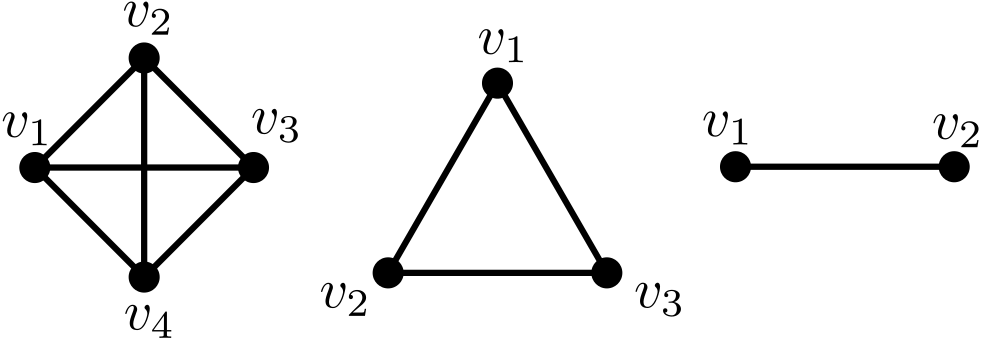
\includegraphics[width=0.55\linewidth]{secGD/figures/grafoCompleto.png}
	\end{center}
	\caption{Em ordem: (a) 4-clique; (b) 3-clique; (c) 2-clique.}
	\label{fig:grafoCompleto}
\end{figure}

Perceba a existência de uma estrutura recursiva nos grafos completos, que se mantém para o caso geral: sendo $G_{K+1} = \{V_G, E_G\}$ um $(K+1)$-clique e $v \in V_G$ um vértice qualquer de $G_{K+1}$, sempre pode-se obter um $K$-clique como o subgrafo induzido $\langle V_G \setminus \{v\}\rangle$. Por conta disso, podemos utilizar essas estruturas como ``blocos básicos de construção'' para planejar uma realização iterativa do grafo como um todo, usando a trilateração para realizar um novo vértice em cada iteração. 




\subsubsection{Realização Iterativa de Grafos Completos}

A seguir, apresenta-se um algorítimo para realizar em $\mathbb{R}^K$ todos os $n$ vértices de um $(n,\frac{n^2 -n}{2})$-grafo completo $G$, com $n > K$, tendo como entrada a posição dos $(K+1)$ primeiros vértices também em $\mathbb{R}^{K}$.
\\

Primeiro, assume-se que exista um $(K+1)$-clique $G_o \subset G$, chamado clique inicial, que conhecemos a realização --- em WSNL, por exemplo, comumente se utiliza nós ancoras como clique inicial \cite{eren2004rigidity, savvides2001dynamic}. Sem perda de generalidade, seja $\{1,\dots,K+1\}$ o conjunto dos vértices que formam a clique inicial $G_o$, com realizações $\{x_1, \dots,x_{K+1}\}$. Seja, também, $N(i)$ o conjunto de vértices adjacentes ao $i$-ésimo vértice. Então, pode-se encontrar uma realização total de $G$ através do Algorítimo~\ref{alg:realizacaoIterativa}. 
\\

\begin{algorithm}[H]
	\label{alg:realizacaoIterativa}
	\tcp{Realize os próximos vértices iterativamente}
	\For{$i\in \{K+2,\dots,n\}$}{
		\tcc{Utilize o $(K+1)$-clique dos $(K+1)$ antecessores imediatos de $i$ para calcular a realização $x_i$. Caso não haja solução, atribuir $\emptyset$}
		$x_i \gets$  Trilateracao$(x_{i-K-1},\dots,x_{i-1})$\;
		\tcp{verifique se $x_i$ é factível com relação as demais distâncias}
		\For{$\{j\in N(i)\ ; \ j<i\}$}{
			\If{$\lVert x_i - x_j\rVert \ne d_{ij}$}{
				\tcp{Sinalizar como não factível e sair do loop}
				$x_i \gets \emptyset$\;
				\textbf{break}\;
			}
		} 
		\If{$x_i = \emptyset$}{
			\tcp{Retornar que a realização não é factível}
			\textbf{return} $\emptyset$\;
		}
	}
	\tcp{Retornar a realização factível}
	\textbf{return} $x$\;
	\caption{RealizacaoIterativa$(G,d, K, x)$ \cite{libertiEDG}}
\end{algorithm}
\vspace{0.5cm}
Note que o Algorítimo~\ref{alg:realizacaoIterativa} tem a complexidade de seu pior caso como $\mathcal{O}(K^3n)$, \textit{i.e.}, para todos os $n$ vértices deve-se resolver um sistema linear $K\times K$ (trilateração). Se não existir realização factível para $G$ em $\mathbb{R}^K$, Algorítimo~\ref{alg:realizacaoIterativa} retorna $\emptyset$.

\begin{definicao}[K-lateração]
	O processo de trilateração iterativa em $\mathbb{R}^K$, descrita pelo Algorítimo~\ref{alg:realizacaoIterativa}, é chamado $K$-\textit{Lateração} \cite{eren2004rigidity}.
\end{definicao}

\subsubsection{Sobre o clique inicial $G_o$ e unicidade \label{sec:go}}
Em um primeiro momento pode parecer pouco razoável necessitar da realização prévia do clique inicial $G_o$. De fato, se o problema possuir apenas $K+1$ vértices, essa solução não faz sentido. Felizmente, em geral, os problemas de estudo costumam ser maiores \cite{carlileGDandAplications}.
\\

É importante perceber que os $K+1$ vértices do clique inicial (já realizados), juntamente com o vértice a se realizar, determinam um simplex no espaço $\mathbb{R}^K$ que, garantida a desigualdade triangular estrita $d_{i,j} < d_{i,u} + d_{u,j}$, para todo $i,j,u \leq K+1$, possui um volume $K$-dimensional $\geq 0$ (veja a Figura~\ref{fig:flatsimplices}) diretamente proporcional ao determinante de Cayley-Menger (como mostrado na Equação~\ref{eq:volumeKdimensionalNSimplex}). Caso esse volume seja zero, que é o que acontece com $(K+2)$-simplex em $\mathbb{R}^K$, tem-se o chamado \textit{Simplex Achatado} (\textit{Flat Simplex}) com no máximo uma realização (como ilustra a Figura~\ref{fig:flatsimplices}, a direita).

\begin{figure}[H]
	\begin{center}
		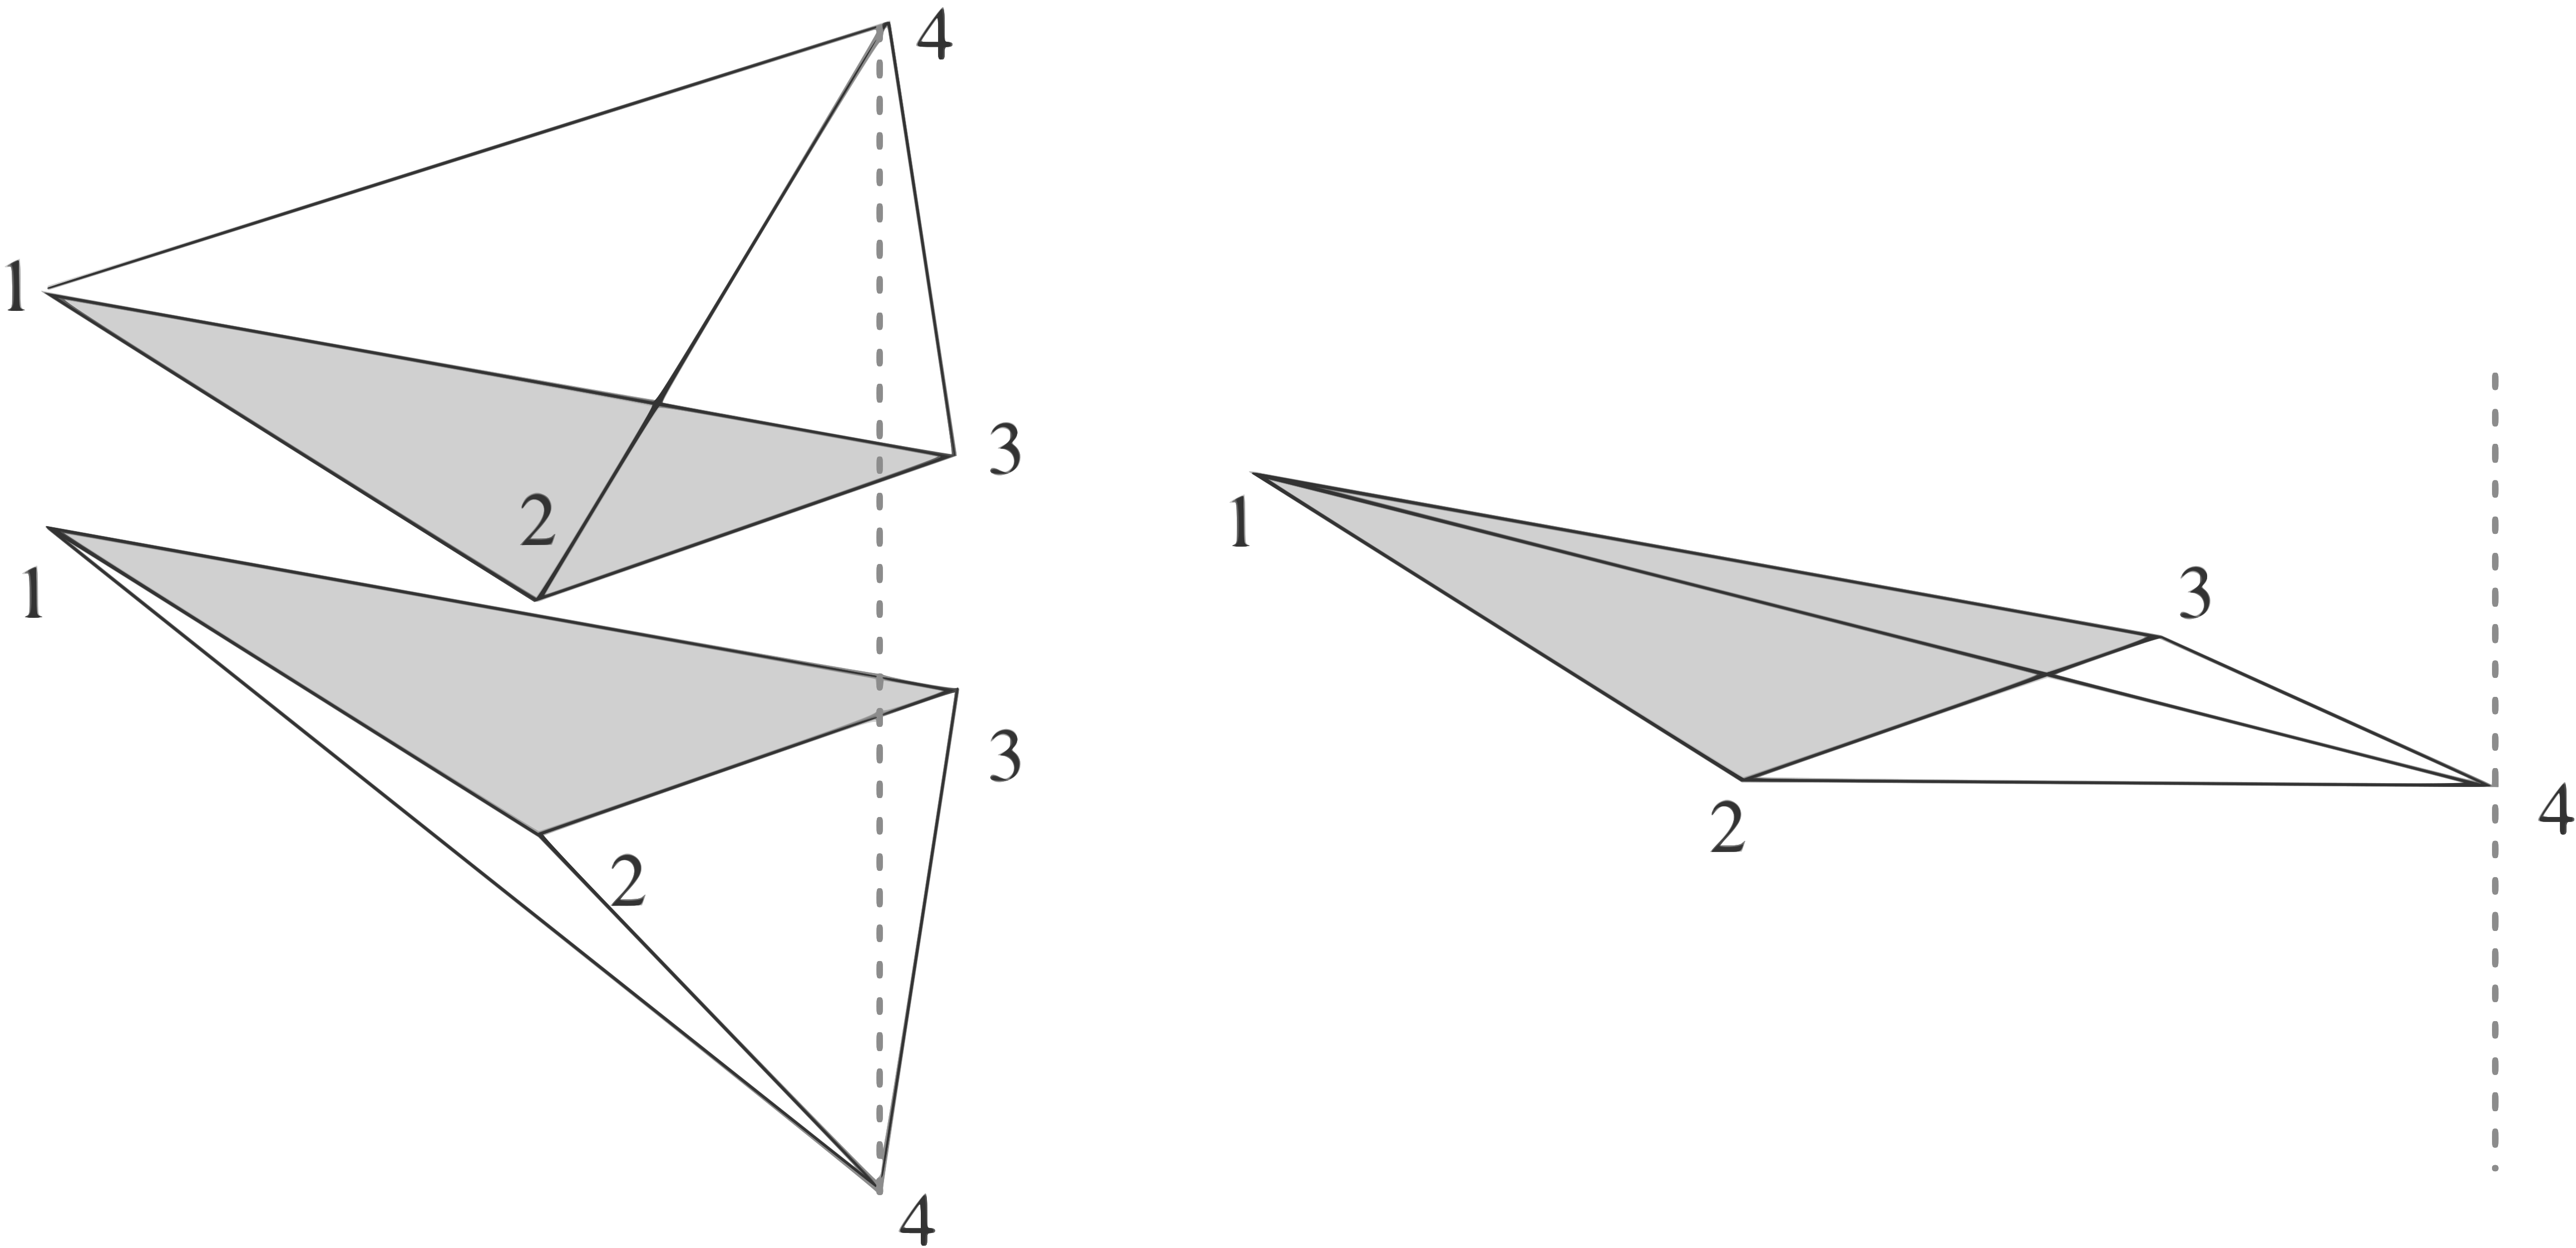
\includegraphics[width=0.7\linewidth]{secGD/figures/flatsimplices.png}
	\end{center}
	\caption{Note que as duas realizações de um mesmo $4$-clique em $\mathbb{R}^3$ (esquerda) são possíveis por respeitarem as distâncias entre os vértices, mas somente uma realização é possível em $\mathbb{R}^{2}$ (direita) \cite{libertiEDG}.}
	\label{fig:flatsimplices}
\end{figure}

De fato, através da relação entre o volume de um simplex com a existência de uma realização para um grafo completo (que pode ou não formar um simplex), permite-se estabelecer condições necessárias e suficientes para a realização de cliques:

\begin{proposicao}
	Uma condição necessária e suficiente para que um $(n+1)$-clique tenha uma realização em $\mathbb{R}^K$, para $K\leq n$, é que todos os determinantes de Cayley-Menger, não nulos, de $m+1$ pontos tenham sinal dado por $(-1)^{m+1}$, para todo $m=1,2,\dots,K$. Além disso, os determinantes de Cayley-Menger de mais de $K+1$ pontos devem ser nulos.
	
	\begin{proof}
		Pode-se encontrar esta demonstração em \cite{correiaCondicoesNecessaESuficiDGPCayleyMenger}
	\end{proof}
\end{proposicao}

\subsubsection{Realizando grafos $K$-laterativos em $\mathbb{R}^K$ \label{sec:oi}}

No Algorítimo~\ref{alg:realizacaoIterativa}, fica implícita a existência de uma ordem no conjunto de vértices $V$ do grafo $G$. Se $G$ é completo, de fato, qualquer ordem $(v_1,\dots,v_n)$ em $V$ é tal que $v_i$ é adjacente a todos os seus antecessores --- isto é, para todo $i>K+1$, tem-se no mínimo os $K+1$ antecessores  necessários para a $K$-lateração. Por outro lado, $G$ não precisa ser necessariamente completo para garantir isso.

\begin{definicao}[Ordem de $K$-lateração]
	Se $<$ é uma ordem em $V$ e $v\in V$ é um vértice qualquer, então $\gamma(v) = \{u\in V \;|\; u<v \}$ é dito conjunto de antecessores de $v$ em relação a $<$ e $\rho(v) = |\gamma(v)|+1$ é dito posto de $v$ em $<$. Dado um grafo $G=(V,E)$, uma ordenação $<$ sobre $V$ é chamada \textit{Ordem de $K$-Lateração} se:
	\begin{enumerate}
		\vspace{-0.2cm}
		\item os primeiros $K+1$ vértices de $<$ induzirem um $(K+1)$-clique $G_o$ em $G$;
		\vspace{-0.2cm}
		\item todo vértice $v$, com $\rho(v) > K+1$, tem $\lvert N_G(v) \bigcap \gamma(v)\rvert \geq K+1$.
	\end{enumerate}
\end{definicao}

Um grafo $G = (V,E)$ é dito \textit{$K$-Laterativo} se há uma ordem de $K$-lateração sobre $V$. Perceba que um grafo $K$-laterativo não precisa ser completo e, mesmo assim, ainda é possível aplicar a $K$-lateração em todo vértice $v \in V$, com posto $\rho(v) >K+1$, como é o caso ilustrado da Figura~\ref{fig:klaterativegraph} para $K = 2$. Seguindo a ordenação $(v_1, v_2, v_3, v_4, v_5)$, pode-se utilizar a $3$-clique $\{v_1,v_2,v_3\}$ para realizar o vértice $v_4$ e utilizar a $3$-clique $\{v_2,v_3,v_4\}$ para realizar o vértice $v_5$.

\begin{figure}[H]
	\begin{center}
		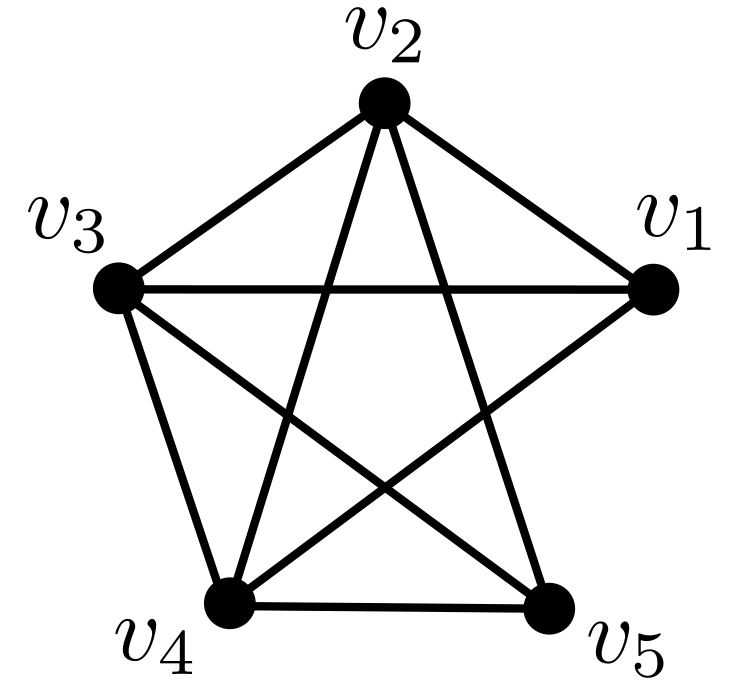
\includegraphics[width=0.26\linewidth]{secGD/figures/klaterativegraph.png}
	\end{center}
	\caption{Grafo $K$-laterativo não completo, de 5 vértices e $K = 2$.}
	\label{fig:klaterativegraph}
\end{figure}

Como a existência de uma ordem de $K$-lateração garante, por definição, que sempre haverá ao menos $K+1$ vértices já realizados antecessores a todo vértice $v \in V$, com $\rho(v) > K+1$, sempre será possível aplicar a $K$-lateração. Assim, um grafo $K$-laterativo possui no máximo uma solução.

\begin{definicao}[Trilaterativo DGP]
	Um DGP $(G,d,K)$ é chamado \textit{Trilaterativo DGP} (TDGP) se uma ordem de $K$-lateração sobre $G$ for dada.
\end{definicao}

Dado um TDGP $(G,d,K)$, seja $\{x_1, \dots,x_{K+1}\}$ o conjunto de realizações dos primeiros $K+1$ vértices em relação a ordem de $K$-lateração. Uma realização $x$ de $G$ em $\mathbb{R}^K$ pode ser encontrada (ou mostrada que não existe) através de uma adaptação do Algorítimo~\ref{alg:realizacaoIterativa}, como mostrado em \cite{libertiEDG}, onde realiza-se os vértices na ordem de $K$-lateração. Além deste algorítimo garantir que no máximo haverá uma solução possível, ele também tem a vantagem de ser em tempo polinomial. Porém, infelizmente, nem sempre é possível obter tal ordem nos vértices e, nesses casos, podemos afrouxar algumas hipóteses objetivando a busca por soluções.

\subsubsection{Realizando grafos $(K-1)$-laterativos em $\mathbb{R}^K$}

Agora trataremos dos casos onde o grafo associado ao problema não possui vértices suficientes para a existência de uma ordem $K$-laterativa. Em particular, estudaremos o caso da realização de um grafo $(K-1)$-laterativo no espaço $\mathbb{R}^K$, que possui uma grande correlação com a classe de problemas moleculares.
\\

Essa correlação vem da estrutura geométrica das proteínas. A cadeia principal de uma proteína é um conjunto $V = \{v_1,\dots,v_n\}$ de átomos com uma certa ordem conveniente induzida pelas ligações químicas da molécula (veja o Apêndice~\ref{ap:biomol}). Conhece-se distância de pares consecutivos $\{v_{i-1},v_i\}$, para todo $i\leq n$, e também conhece-se o ângulo de ligação entre três átomos consecutivos $(v_{i-2},v_{i-1}, v_i)$. Dessa forma, pode-se calcular a distância entre dois átomos separados por duas ligações, i.e., de pares ${v_{i-2},v_i}$, ao se construir o triângulo formado pelos dados de distâncias e ângulos. Então, se a distância de pares $\{v_{i-3},v_i\}$ separados por três ligações não puderem ser determinadas (usando, por exemplo dados de RMN), então acontece que existe uma ordem alternativa para os vértices de forma que $v_i$ seja sempre adjacente a pelo menos os últimos três predecessores \cite{libertiEDG}.

Dessa forma, cadeias principais de proteínas podem ser modeladas por grafos $2$-laterativos (i.e., cada vértice é adjacente a pelo menos 3 antecessores), que precisam ser realizadas no espaço $\mathbb{R}^3$. Porém, encontrar essa ordem nos vértices da molécula pode não ser trivial. O problema de encontrar essa ordem é definido como Problema da Ordem de Discretização (ou DVOP) e está relacionado com encontrar uma ordem de $(K-1)$-lateração. É importante mencionar que o DVOP é um problema NP-Completo \cite{carlile:dvopComplexity}. Entretanto, uma ordem pode ser construída manualmente, assim como feito em \cite{carlile:MinimalOrder,douglasSideChainOrder}. 

\begin{definicao}[MDGP Discretizável]
	O MDGP Discretizável (DMDGP) é um MDGP com uma ordenação em seus vértices tal que
	\begin{enumerate}
		\vspace{-0.2cm}
		\item (discretização). para todo par de vértices $i,j\in V$ com $1\leq \norm{i-j} \leq 3$, temos $\{i,j\} \in E$;
		\vspace{-0.2cm}
		\item (não-colinearidade). os valores de distância entre cada tripla de vértices consecutivos $i-2,i-1$ e $i$ na ordenação satisfazem a desigualdade triangular estrita $$d_{i-2,j}<d_{i-2,i-1}+d_{i-1,i}, \text{ para todo } i\geq 3$$.
	\end{enumerate}
\end{definicao}

A seguir apresenta-se uma ordenação manual nos vértices de uma proteína chamada Hand-Crafted Order (ou, HC Order), proposta por Lavor \textit{et. al.} \cite{carlile:MinimalOrder}, que respeita a definição do DMDGP.

\subsubsection*{HC Order\label{sec:hc}}
Seja $G = (V, E, d)$ o grafo associado a cadeia principal de uma proteína $(\{N^k,\ $ $ C^{k}_\alpha,C^k\}$, para $k = 1,\dots,p)$, incluindo os átomos de oxigênio $O^k$, ligados ao $C^k$, e átomos de hidrogênio $H^k$ e $H^{k}_\alpha$, ligados ao $N^k$ e $C^{k}_\alpha$, respectivamente (conforme Figura ~\ref{fig:hcVO}, a esquerda, onde $p = 3$).

\begin{figure}[H]
	\begin{center}
		\includegraphics[width=1\linewidth]{figures/proteinsGroup-eps-converted-to.pdf}
	\end{center}
	\caption{A esquerda, o esboço da cadeia principal expandida. No centro, uma representação da ordem HC. A direita, uma representação do grafo associado a ordenação.}
	\label{fig:hcVO}
\end{figure}

Define-se a ordem HC como:

\begin{minipage}{0.532\linewidth}
	$$
	hc = \{ N^1, H^1, H^{1'}, C_{\alpha}^1, N^1, H_{\alpha}^1, C^1, C_{\alpha}^1, \dots,
	$$
	
\end{minipage}
%\vspace{-0.1cm}
$$
H^i, C_{\alpha}^i, O^{i-1}, N^i, H^i, C^{i}_\alpha, N^i, H^{i}_\alpha, C^i, C_{\alpha}^i,\dots,
$$

\hspace{4.5cm}
\begin{minipage}{0.532\linewidth}
	\vspace{-0.7cm}
	$$
	H^p, C_{\alpha}^p, O^{p-1}, N^p, H^p, C^{p}_\alpha, N^p, H^{p}_\alpha, C^p, C_{\alpha}^p, O^p, C^p, O^{p'}\}
	$$
\end{minipage}
\\

Onde, como na Figura ~\ref{fig:hcVO}, $i = 2, \dots, p-1$, $H^{1'}$ é o segundo hidrogênio ligado ao $N^1$ e $O^{p'}$ é o segundo oxigênio ligado ao $C^p$.	
\\


Toda distância entre hidrogênios relativamente próximos (representados por vértices tracejados no grafo da Figura~\ref{fig:hcVO}) --- inclusive entre $H_\alpha^{i-1}$ e $H^{i}$ --- são dados pelos experimentos de RMN. Também, para termos ao menos um grafo 2-laterativo, no átomo $H^i$, precisamos ter conhecimento do plano mostrado na Figura ~\ref{fig:peptidica} (veja Apêndice~\ref{ap:biomol}), que diz que os átomos em torno da ligação peptídica são coplanares --- e, por tanto, pode-se descobrir a distância entre o $H^i$ e $C_\alpha^{i-1}$ através dos cossenos.
\\

A ordenação HC gera uma estrutura muitíssimo interessante para se trabalhar. De fato, por garantir que sempre tenhamos pelo menos um 3-clique em todo átomo com posto maior que três, ao tentarmos localizar o quarto átomo estamos realizando um 4-clique no $\mathbb{R}^3$ e, como vimos anteriormente, essa situação descreve a realização de um $4$-simplex no $\mathbb{R}^3$ que pode ter duas soluções (veja Figura~\ref{fig:flatsimplices}). Na verdade, é pela existência do $K$-simplex estar relacionado a desigualdade triangular que o DMDGP carrega ela em sua ordenação. A interpretação geométrica disso é que estamos calculando a realização do próximo átomo da sequência $v_i$ com $i \geq 4$, utilizando a interseção das 3 esferas centradas nos três átomos anteriores $v_{i-3}, v_{i-2}$ e $v_{i-1}$ (já realizados) e com os respectivos raios iguais as distâncias $d_{i,i-3}, d_{i,i-2}$ e $d_{i,i-1}$ para o átomo $i$ que se está tentando localizar. 
Essas intersecções tem três possibilidades associadas (veja Figura ~\ref{fig:esferas}): Ou não temos nenhum ponto de interseção entre elas (isso não acontece por definição no DMDGP); ou existe um ponto (também fere a definição e, de fato, isso não acontece nas proteínas) ou existem dois pontos onde as esferas se interceptam (o caso geral proteico).

\begin{figure}[H]
	\begin{center}
		\includegraphics[width=0.8\linewidth]{figures/esferas.png}
	\end{center}
	\caption{Interseção de três esferas \cite{carlileBook31Coloquio}.}
	\label{fig:esferas}
\end{figure}

Assim, perceba que além da ordenação dos vértices garantir a finitude do conjunto solução do problema, como sempre temos duas possibilidades de realização, ela também organiza o espaço onde devemos fazer a busca por uma solução. Na verdade, a ordem induz uma estrutura de \textit{árvore binária} no espaço de busca \cite{fidalgotese}.

\subsection{\textit{Branch-and-Prune} \label{sec:bp}}

Apresentado em 2007 \cite{carlile:BP}, por Leo Liberti, Carlile Lavor e Nelson Maculan, este algorítimo (também chamado BP) consiste em uma estratégia numérica recursiva, que resolve o DMDGP eficientemente utilizando uma busca combinatória no espaço de busca de soluções, onde realiza-se vértice por vértice do sistema, seguindo a ordem dada, ``podando'' --- isto é, descartando --- todo sub-conjunto solução do sistema que não esteja de acordo com as informações pré-estabelecidas. Desde que ele foi publicado, tem se verificado tanto sua beleza matemática, quanto a sua eficiência numérica-computacional para resolver problemas em Geometria de Distâncias.

\subsubsection{Representações de Átomos em Coordenadas Internas\label{sec:bi}}
As coordenadas internas de uma proteína são definidas pela distância entre os átomos $d_{1,2}, ..., d_{n - 1,n}$, pelo ângulo planar $\theta_{1,3}, ...,\theta_{n - 2,n}$ (formados por 3 átomos consecutivos) e pelos ângulos de torção $\omega_{1,4}, ..., \omega_{n-3,n}$ (formado por 4 átomos consecutivos), conforme ilustrado na Figura ~\ref{fig:angulos}. O ângulo de torção é definido entre os planos formados pelos átomos $i-3,i-2,i-1$ e $i-2,i-1,i$, respectivamente. Assim, temos que $\omega$ varia no intervalo $[0,2\pi]$ e $\theta$ de $[0,\pi]$ --- assim como em um sistema de coordenadas esféricas. As distâncias entre os átomos unidos por ligações covalentes são da ordem de 1,5\AA. 

\begin{figure}[H]
	\begin{center}
		\includegraphics[width=0.6\linewidth]{figures/genericConf-4Fidalgo.png}
	\end{center}
	\caption{Ângulos planos e de torção}
	\label{fig:angulos}
\end{figure}

Note que, usando os valores de distâncias das cliques $\{ v_{i-3}, v_{i-2} , v_{i-1}, v_i \}$ garantidas pelo DMDGP, temos gratuitamente todas as distâncias entre átomos consecutivos $d_{1,2}, \dots, d_{n-1, n}$, donde podemos obter pela lei dos cossenos os ângulos planos $\theta_{1,3}, \dots, \theta_{n-2, n}$ 
\begin{equation}
	%
	\cos(\theta_{i-2,i}) 
	= 
	\dfrac{d^{2}_{i-2,i-1} + d^{2}_{i-i,i} - d^{2}_{i-2,i}}{2d_{i-2,i-1}d_{i-1,i}}
	%
	\hspace{0.5cm} \mbox{  e  } \hspace{0.5cm}
	%
	\sin(\theta_{i-2,i}) = \sqrt{1 - \cos^{2}(\theta_{i-2,i})},
	%
	\label{eqcostheta}.
\end{equation} 

Já o cosseno de um ângulo de torção (também chamado diedral) pode ser dado em função de distâncias euclidianas e ângulos planos \cite{carlileTese}. Assim, sejam as triplas $\{ v_{i-3} , v_{i-2} , v_{i-1} \}$ and $\{ v_{i-2} , v_{i-1},v_{i} \}$, para $i \in \{ 4 , \hdots , n \}$, os cossenos dos ângulos diedrais são dados por
\begin{equation}
	%
	\cos( \omega_{i-3,i} ) = 
	\dfrac{ 2d^{2}_{i-2,i-1} 
		\left( d^{2}_{i-3,i-2} + d^{2}_{i-2,i} - d^{2}_{i-3,i} \right) - (\tilde{d}_{i-3,i-1})(\tilde{d}_{i-2,i}) }
	{ \sqrt{\left( 4d^{2}_{i-3,i-2}d^{2}_{i-2,i-1} - \tilde{d}^{2}_{i-3,i-1}\right) 
			\left( 4d^{2}_{i-2,i-1}d^{2}_{i-1,i} - \tilde{d}^{2}_{i-2,i} \right)} },
	%
	\label{eqcosomega}
	%
\end{equation}
com $\tilde{d}_{i-3,i-1} = d^{2}_{i-3,i-2} + d^{2}_{i-2,i-1} - d^{2}_{i-3,i-1}$ e $\tilde{d}_{i-2,i} = d^{2}_{i-2,i-1} + d^{2}_{i-i,i} - d^{2}_{i-2,i}$. Porém, dessa forma, não temos como definir exatamente o seno desse ângulo. Só podemos fazer $\mbox{sen}(\omega_{ijkl}) = \pm\sqrt{1 - \cos^2(\omega_{ijkl})} \label{eq:senOmega}$. Isso é, sempre possuímos dois possíveis ângulos associados ($\omega_{i-3, i}^0$ e $\omega_{i-3,i}^1$). Daí a decisão binária ilustrada na Figura ~\ref{fig:torcao} para as duas posições possíveis ($\mathbf{x}_i^0$ e $\mathbf{x}_i^1$) para o vértice $i\geq 4$.

\begin{figure}[H]
	\begin{center}
		\includegraphics[width=0.45\linewidth]{figures/simetria.png}
	\end{center}
	\caption{Duas possibilidades para o ângulo de torção.}
	\label{fig:torcao}
\end{figure}

Por tanto, conseguimos definir todo o problema a partir das coordenadas internas. Como nosso objetivo é obter as posições tridimensionais de cada átomo, nosso problema se restringiu em transformar as coordenadas internas em cartesianas. Para isso, utiliza-se uma série de operações lineares baseadas em \cite{thompsonBi}.
\\

Consideremos que as coordenadas do ponto $\mathbf x_{i} \in\mathbb{R}^3,i= 1, ...,n $ são dadas por $(x_{i1},x_{i2},x_{i3})$, temos:

$$
\begin{bmatrix}
	x_{i1}\\ 
	x_{i2}\\ 
	x_{i3}\\ 
	1
\end{bmatrix}
= B_{1}B_{2}\cdots B_{i}\begin{bmatrix}
	0\\ 
	0\\ 
	0\\ 
	1
\end{bmatrix},
$$
onde
$$
B_1\: =\:
\begin{bmatrix}
	1 & 0 & 0 & 0\\ 
	0 & 1 & 0 & 0\\ 
	0 & 0 & 1 & 0\\ 
	0 & 0 & 0 & 1
\end{bmatrix},\:\:\:
\: B_2\: =\:
\begin{bmatrix}
	-1 & 0 & 0 & -d_{1,2}\\
	0 & 1 & 0 & 0\\ 
	0 & 0 & -1 & 0\\ 
	0 & 0 & 0 & 1
\end{bmatrix},
$$
$$
B_3\:=\:
\begin{bmatrix}
	-\cos\theta_{1,3} & -\mbox{sen}\theta_{1,3} & 0 & -d_{2,3}\cos\theta_{1,3}\\ 
	\mbox{sen}\theta_{1,3} & -\cos\theta_{1,3} & 0 & d_{2,3}\mbox{sen}\theta_{1,3}\\ 
	0 & 0 & 1 & 0\\ 
	0 & 0 & 0 & 1
\end{bmatrix}
$$
e
$$
B_i\:=\:
\begin{bmatrix}
	-c_{\theta_{i}} & -s_{\theta_{i}} & 0 & -d_{i-1,i}c_{\theta_{i}}\\ 
	s_{\theta_{i}}c_{\omega_{i}} & -c_{\theta_{i}}c_{\omega_{i}}
	& -s_{\omega_{i}} & d_{i-1,i}s_{\theta_{i}}c_{\omega_{i}}\\ 
	s_{\theta_{i}}s_{\omega_{i}} & -c_{\theta_{i}}s_{\omega_{i}} & c_{\omega_{i}} & d_{i-1,i}s_{\theta_{i}}s_{\omega_{i}}\\ 
	0 & 0 & 0 & 1
\end{bmatrix}
$$
dado $s_{\theta_{i}}=\mbox{sen} (\theta_{i-2, i}),\: c_{\theta_{i}}=\cos (\theta_{i-2, i}),\: s_{\omega_{i}}=\mbox{sen} (\omega_{i-3, i}),\: c_{\omega_{i}}=\cos (\omega_{i-3, i})$. Em $B_i$, $i=4, ..., n$.
\\

Perceba que $B_i$ (chamada \textit{Matriz de Torção}) é a matriz que engloba todas as operações necessárias para encontrar a i-ésima realização do i-ésimo átomo da molécula, tendo conhecimento de todas as matrizes $B_j$ $\forall j < i$. Como é de grande importância o entendimento de tais operações que formam a $B_i$, segue a separação das suas transformações em termos de matrizes de rotação $R_v(\theta)$, que descreve a rotação de $\theta$ ao redor do eixo definido por $\langle v\rangle$, e uma matriz de translação $T_x(d)$ no espaço homogêneo que descreve a translação $d$ no eixo $x$:
$$
B_i=R_{x}(w_{i-3,i})\cdot R_{x}(\pi)\cdot R_{z}(\theta_{i-2,i})\cdot R_{y}(-\pi)\cdot T_{x}(d_{i-1,i}).
$$

Note também que fixando os comprimentos das ligações covalentes $d_{1,2},d_{2,3}$ e o valor do ângulo plano $\theta_{1,3}$, os três primeiros átomos terão as coordenadas dadas por
$$
x_1\:=\:
\begin{bmatrix}
	0\\ 
	0\\  
	0
\end{bmatrix},\:\:\:
x_2\:=\:
\begin{bmatrix}
	-d_{1,2}\\ 
	0\\  
	0
\end{bmatrix},\:\:\:
x_3\:=\:
\begin{bmatrix}
	-d_{1,2}+d_{2,3}\cos\theta_{1,3}\\ 
	d_{2,3}\mbox{sen}\theta_{1,3}\\  
	0
\end{bmatrix}.
$$

\begin{figure}[H]
	\begin{center}
		\includegraphics[width=0.6\linewidth]{figures/inicializationgray.eps}
	\end{center}
	\caption{Inicialização do BP}
	\label{fig:inicializacao}
\end{figure}	

\subsubsection*{O algorítimo BP}

Como todo algorítimo, esse possui um conjunto de entradas e saídas.
\begin{description}
	\item[Entradas:] O grafo $G(V, E, d)$ que define o DMDGP --- onde possuímos uma ordenação para $V$ --- e mais um escalar $\varepsilon \in \mathbb{R}$ que da a tolerância aceita no algoritmo (pois o BP não é um método exato, encontrando apenas soluções distantes a menos de $\varepsilon$ das reais).
	
	Para facilitar a utilização do algorítimo, também faremos uma distinção dos vértices que compõem o conjunto $E$: Sejam os subconjuntos $E_{d}, E_p \subset E$, tal que $E = E_{d} \cup E_{p}$ --- denominados como, respectivamente, \textit{arestas de discretização} e \textit{arestas de poda} ---, onde
	
	\begin{center}
		$E_{d} = \{\{v_i,v_j\} \in E : |i-j|\leq 3\}$ e $E_{p} = E - E_d$.
	\end{center}
	
	\item[Saídas:] Uma árvore binária $T$, onde cada nó de nível $i$ da árvore é uma realização possível do vértice $v_i \in V$, de tal forma que o caminho $C \subset T$ partindo da raiz (primeiro nó) até uma folha de nível $n = |V|$ da árvore seja uma solução para o problema, isto é, um conjunto de realizações de todos os átomos da molécula.
\end{description}

São três fases que definem o algoritmo: Inicialização, \textit{Branching} e \textit{Pruning} \cite{fidalgotese}.

\subsubsection*{Inicialização}
Esta etapa se preocupa com a inicialização da estrutura. Ela define a realização dos três primeiros átomos $v_1, v_2$ e $v_3 \in V$ da sequência, que são posicionados nas respectivas posições $x_1, x_2$ e $x_3 \in \mathbb{R}^3$, utilizando as operações contidas nas matrizes $B_1, B_2$ e $B_3$. 

Essas três primeiras posições estão associados biunivocamente com os três primeiros nós da arvore de busca $T$ (representada por um grafo), que também é iniciada, conforme Figura ~\ref{fig:bp1}

\begin{figure}[H]
	\begin{center}
		\includegraphics[width=0.035\linewidth]{figures/bp1.png}
	\end{center}
	\caption{Inicialização de T \cite{fidalgotese}.}
	\label{fig:bp1}
\end{figure}

\subsubsection*{\textit{Branching}}
Essa etapa está associada com o processo de ``ramificação'' de $T$ \cite{fidalgotese}. Ou seja, supondo que já foram realizados os vértices $v_1, \dots, v_{i-1}$ (onde $3 < i< |V|$), repeitando a ordenação em $V$, nosso objetivo é obter a realização $x_i = (x_{i1}, x_{i2}, x_{i3}) \in \mathbb{R}^3$ do vértice $v_i \in V$.

Para isso, basta calcularmos o produto matricial
$$
\begin{bmatrix}
	x_{i1}\\ 
	x_{i2}\\ 
	x_{i3}\\ 
	1
\end{bmatrix}
= C_{i}\begin{bmatrix}
	0\\ 
	0\\ 
	0\\ 
	1
\end{bmatrix},
$$
onde $C_i = C_{i-1}B_i = \prod_{j=1}^{i}B_j$ é dita o \textit{produto acumulado} das matrizes de torção $B_j$. O conceito de ramificação vem do fato de sempre temos duas matrizes de torção $B_j^0$ e $B_j^1$ associadas a cada vértice $v_j$ (por conta dos diferentes ângulos diedrais). A cada matriz de torção temos como resultado um novo conjunto de realizações, que se visualiza como um novo ramo de $T$.

Ilustramos esse processo na Figura ~\ref{fig:ramificacoes}, que presume um DMDGP com $|V| = 6$. Ou seja, obtemos $2^{6-3} = 2^3 = 8$ possíveis soluções, dadas pelas suas 6 ramificações.

\begin{figure}[H]
	\begin{center}
		\includegraphics[width=0.45\linewidth]{figures/ramificacoes.png}
	\end{center}
	\caption{Árvore $T$ completa de uma instância DMDGP com 6 vértices \cite{fidalgotese}.}
	\label{fig:ramificacoes}
\end{figure}

Fica claro aqui que o processo de ramificação garante que, no máximo, existem $2^{n-3}$ soluções possíveis para o problema. Isso colabora com a enumerabilidade e finitude do conjunto solução do problema, porém, também mostra que o número de soluções cresce de uma forma exponencial com o crescimento da molécula.

\subsubsection*{\textit{Pruning}}
Essa etapa tem como função diminuir drasticamente o conjunto solução do problema. Conseguimos isso ao classificar os diferentes ramos de $T$ como factíveis ou não e, então, ``podando'' os infactíveis.  

Como já discutimos antes, para calcular as matrizes de torção da etapa anterior só precisamos dos dados do 3-clique garantido pelas hipóteses do DMDGP, ou seja, das distâncias $d_{i,i-3}, d_{i,i-2}$ e $d_{i,i-1}$ associadas aos elementos de $E_d$. Com isso, todas as distâncias associados aos elementos de $E_p$ podem ser consideradas como dados adicionais para o problema. 
Isso é, de posse de uma distância extra $d_{i,j}$, recairíamos na realização de um subgrafo $K$-laterativo em $\mathbb{R}^K$, que vimos ter no máximo uma solução. Do ponto de vista geométrico, isso representa a inserção de uma esfera extra àquelas três definidas pelo 3-clique (veja Figura ~\ref{fig:quatroesferas}) e, como a interseção de quatro esferas no $\mathbb{R}^3$ é no máximo 1 ponto, podemos descartar alguma solução.

\begin{figure}[H]
	\begin{center}
		\includegraphics[width=0.35\linewidth]{figures/quatroesferas.png}
	\end{center}
	\caption{Interseção de quatro esferas no $\mathbb{R}^3$ \cite{carlileBook31Coloquio}.}
	\label{fig:quatroesferas}
\end{figure}

E é este o princípio da factibilidade de um ramo. Sempre que estamos na etapa de \textit{Branching} --- ou seja, calculando uma realização $\mathbf x_i$ de $v_i$ a partir de uma matriz de torção ---, podemos verificar se existe uma distância extra associada a algum elemento $\{v_i,v_j\} \in E_p$ tal que $j < i$ e, caso exista, podemos verificar se $|x_i - x_j| < \varepsilon$. Caso for, significa que o ramo passou pela tolerância e é factível. Caso não for, podemos descartar (podar) todas as soluções associadas a sub-árvore definida por aquele ramo.

A etapa de \textit{pruning} é ilustrada na Figura ~\ref{fig:poda} (adaptada de \cite{fidalgotese}). Dando continuidade ao exemplo da Figura ~\ref{fig:ramificacoes}, agora temos $E_p = \{\{v_1,v_5\},\{v_2,v_6\}\}$, o que nos permitiu testar a factibilidade dos ramos associados ao $v_5$ e ao $v_6$ e podar os infactíveis, diminuindo consideravelmente o conjunto solução.

\begin{figure}[H]
	\begin{center}
		\includegraphics[width=0.45\linewidth]{figures/prune.png}
	\end{center}
	\caption{Árvore $T$ de um DMDGP de 6 vértices com a poda evidenciada.}
	\label{fig:poda}
\end{figure}

Perceba que o crescimento exponencial de soluções ($2^{n-3}$) da etapa de \textit{branching} está associado com o DMDGP ser um problema \textbf{NP}-Difícil. Por conta disso é que esse algorítimo tem tanta beleza associada, isto é, apesar da grande complexidade de se resolver o problema original, o BP pode encontrar rapidamente essas soluções.
\\

Mas uma dúvida ainda é importante: E se o conjunto $E_p = \emptyset$? Neste caso, $E = E_d$ e, portanto, todas as posições finais são factíveis trivialmente. Dessa forma, todas as $2^{n-3}$ realizações encontradas durante a etapa de \textit{branching} representam soluções possíveis para o DMDGP, o que, é claro, é o nosso pior caso, pois o BP precisa continuar a exploração de todos os $2^{n-3}$ nós de $T$. 

Por outro lado, se utilizarmos a ordenação HC como ordem que define o DMDGP, nós garantimos que $E_p \neq \emptyset$. Essa é uma das vantagens dessa ordenação. Na verdade, muito mais do que não vazio, graças as propriedades geométricas das proteínas apresentadas em \cite{carlile:MinimalOrder}, pode-se enunciar o seguinte resultado: 

\begin{teorema}
	Usando a ordenação HC, considerando que todos os ângulos e distâncias das ligações atômica estão fixadas nos seus valores de equilíbrio energético (essa é conhecida como \textit{hipótese de geometria rígida}), que os átomos ao redor das ligações peptídicas formam um plano, que as posições possíveis para $C_\alpha^1$ e $C^j$ (com $j = 1, \dots,p$) são únicas --- devido a propriedade quiral do tetraedro formado por $\{N^1, H^1, H^{1\prime}, C_\alpha^1\}$ e $\{C_\alpha^j, N^j, H^j_\alpha,C^j\}$ --- e, dado o conjunto de distâncias entre os pares de átomos de hidrogênio
	$$\{H^{1\prime}, H^1_\alpha\}, \dots, \{H_\alpha^{i-1}, H^i\}, \{H^i, H^i_\alpha\}, \{H^i_\alpha, H^{i+1}\}, \dots, \{H^p, H^p_\alpha\}$$
	(onde $i = 2, \dots, p-1$ e $p$ é o número de aminoácidos que compõem a proteína), as ramificações na árvore de busca só ocorrem em átomos de hidrogênio dados por
	$$\{H_\alpha^1, \dots, H^i, H_\alpha^i, \dots, H^p, H_\alpha^p\}.$$	
\end{teorema}

\subsubsection{O Algorítimo}
Agora que a ideia por trás do BP está desenvolvida nos três passos anteriores (inicialização, \textit{branching} e \textit{pruning}) podemos apresenta-lo formalmente como um algorítimo de uma função recursiva, como segue.
\\

\begin{algorithm}[H]
	\uIf{$i\leq n-1$}{
		Calcule as matrizes de torção $B_i^1$ e $B_i^2$;\\
		Recupere a matriz de torção acumulada $C_{i-1}$ referente ao nó-pai $P(v)$;\\
		Calcule as próximas matrizes de torção acumuladas $C_i \gets C_{i-1}B_i^1$ e $C_i^\prime \gets C_{i-1}B_i^2$;\\
		Utilize-as para calcular as posições $x_i \gets C_iy$ e $x_i^\prime \gets C_i^\prime y$;\\
		$\lambda \gets 1; \rho \gets 1$;\\
		\ForEach{$\{v_j,v_i\} \in E_p$ com $j<i$}{
			\If{$(||x_j - x_i||^2 - d_{ij}^2)^2 > \varepsilon$}{
				$\lambda \gets 0$;	
			}	
			\If{$(||x_j - x_i^\prime||^2 - d_{ij}^2)^2 > \varepsilon$}{
				$\rho \gets 0$;	
			}	
		}
		
		\uIf{$\lambda = 1$}{
			Crie um nó $z$, armazenando $C_i$ e $x_i$ e fazendo $P(z) \gets v$ e $L(v) \gets z$;\\
			$T \leftarrow T \cup \{z\}$;\\
			BranchAndPrune($T,z,i+1$);
		}\Else{
			$L(v) \gets$ PRUNED;
		}
		\uIf{$\rho = 1$}{
			Crie um nó $z^\prime$, armazenando $C_i^\prime$ e $x_i^\prime$ e fazendo $P(z^\prime) \gets v$ e $R(v) \gets z^\prime$;\\
			$T \leftarrow T \cup \{z^\prime\}$;\\
			BranchAndPrune($T,z^\prime,i+1$);
		}\Else{
			$R(v) \gets$ PRUNED;			
		}	
	}
	\Else{
		\tcc{Solução está armazenada nos nós-pais de $n$ a $1$, em busca retrocedida}
		return $T$
	}
	\caption{BranchAndPrune($T,v,i$) \cite{fidalgotese} \cite{carlile:BP}}
\end{algorithm}